\section{Quadrilateral}
\label{sec:Quad}

\begin{figure}[!ht]
\begin{center}
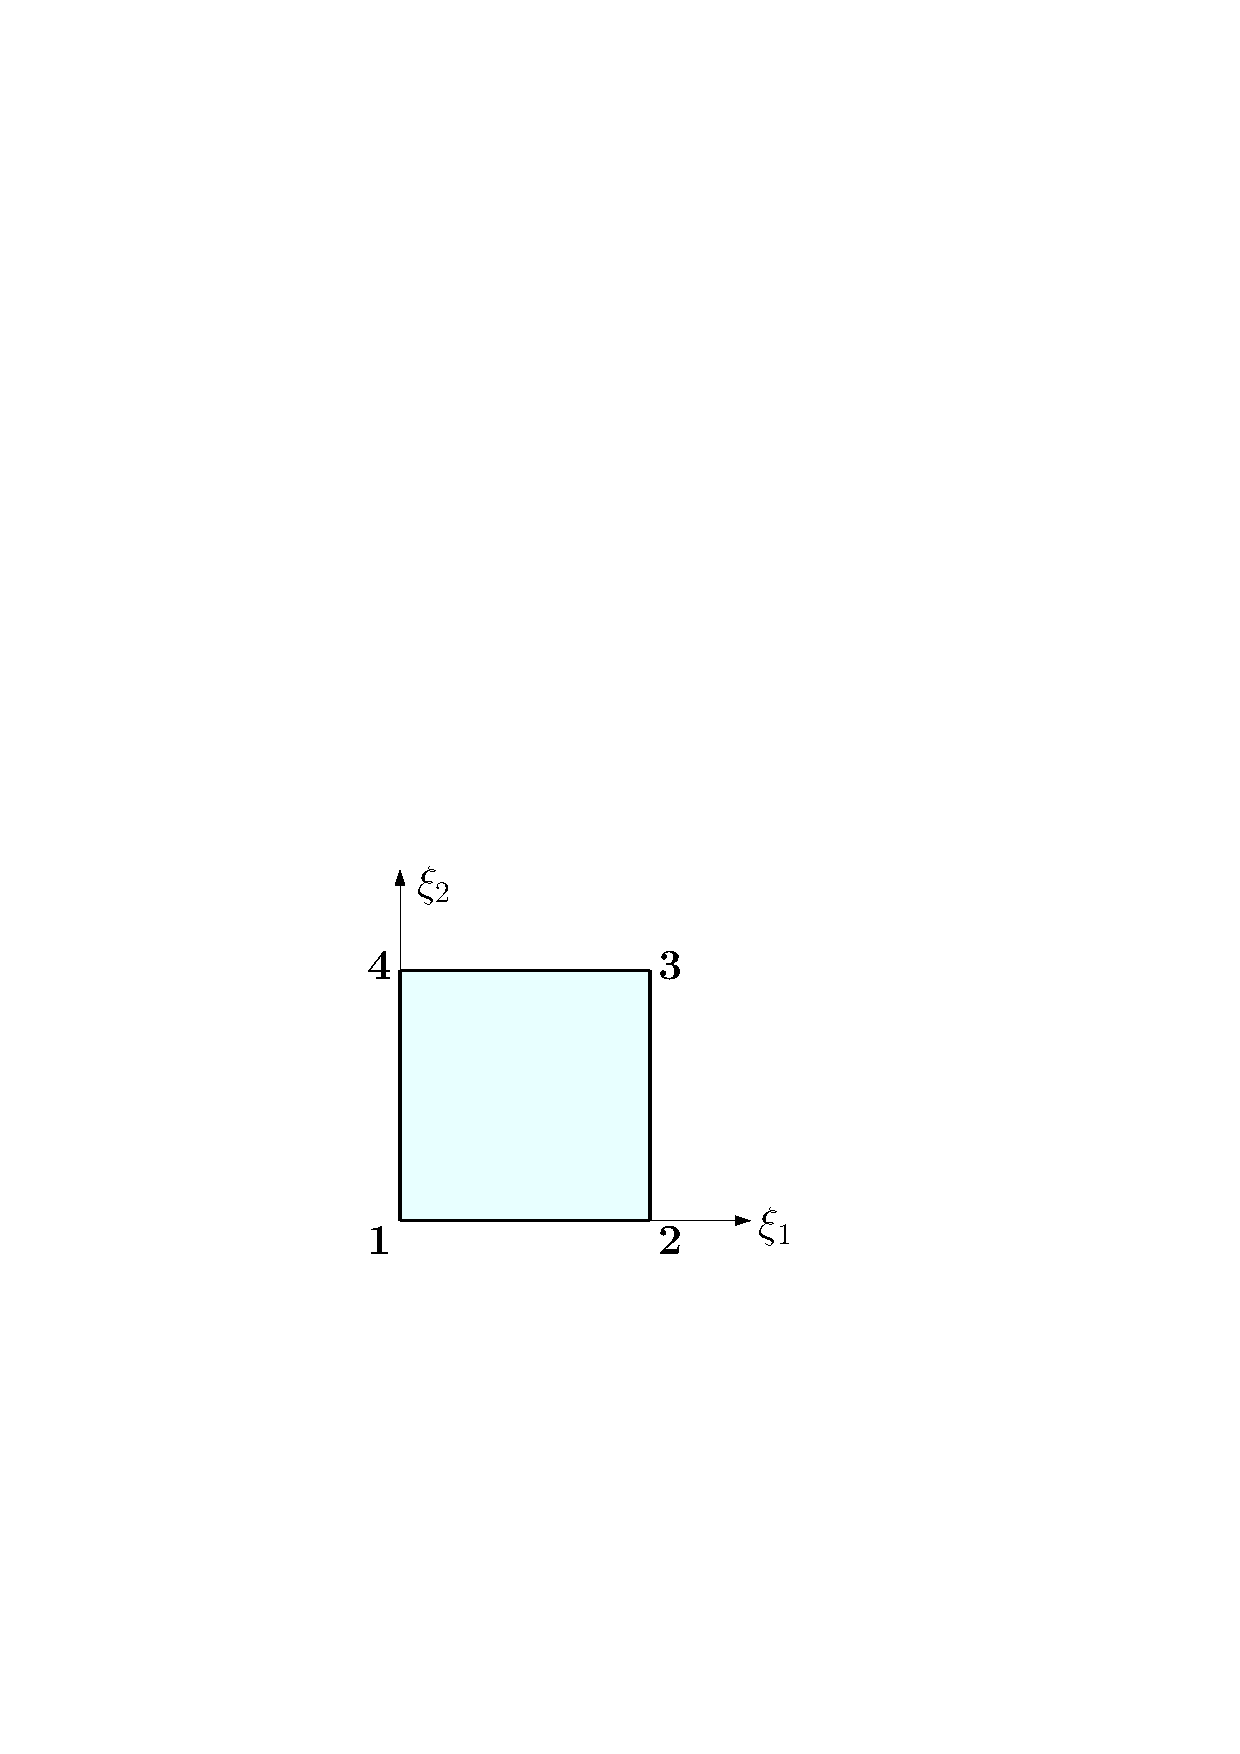
\includegraphics[scale=0.5]{./figures/MasterQuad.pdf}
\caption{Master quadrilateral with numbered vertices.}
\label{fig:MasterQuad}
\end{center}
\end{figure}

The master element for quadrilaterals, which is $(0,1)^2$, is shown in Figure \ref{fig:MasterQuad} in $\xi=(\xi_1,\xi_2)$ space.
The master quadrilateral is clearly a Cartesian product of two segments.

Due to the product structure, there are \textit{two} pairs of 1D affine coordinates:
\begin{equation}
    \begin{alignedat}{4}
        \mu_0(\xi_1)&=1-\xi_1\,,\quad \mu_1(\xi_1)=\xi_1\,\qquad&\Rightarrow\qquad
            \nabla\mu_0(\xi_1)&=\Big(\begin{smallmatrix}-1\\[2pt]0\end{smallmatrix}\Big)\,,\quad
                \nabla\mu_1(\xi_1)=\Big(\begin{smallmatrix}1\\[2pt]0\end{smallmatrix}\Big)\,,\\
        \mu_0(\xi_2)&=1-\xi_2\,,\quad \mu_1(\xi_2)=\xi_2\,\qquad&\Rightarrow\qquad
            \nabla\mu_0(\xi_2)&=\Big(\begin{smallmatrix}0\\[2pt]-1\end{smallmatrix}\Big)\,,\quad
                \nabla\mu_1(\xi_2)=\Big(\begin{smallmatrix}0\\[2pt]1\end{smallmatrix}\Big)\,.
    \end{alignedat}
\end{equation}
These will be used explicitly or implicitly in the formulas that follow.

Again, vertex $a$ is denoted by $v_a$, so that $v_1=(0,0)$, $v_2=(1,0)$, $v_3=(1,1)$ and $v_4=(0,1)$.
These vertices are related to the affine coordinates just as in 1D.
For example, over edge 12 (or edge 43), $\mu_0(\xi_1)$ is the weight related to $v_1$, while $\mu_1(\xi_1)$ is the weight related to $v_2$ (and similarly with $v_4$ and $v_3$).
Indeed, given a point $(\xi_1,0)$ on edge 12, it holds that $(\xi_1,0)=\mu_0(\xi_1)v_1+\mu_1(\xi_1)v_2$.
The same way, $\mu_0(\xi_2)$ is related to $v_1$ in edge 14, so that $v_1$ is linked to both $\mu_0(\xi_1)$ and $\mu_0(\xi_2)$.
A similar assertion holds for each vertex, where each is linked to \textit{two} affine coordinates.
Now, looking at the edges, note that $\mu_0(\xi_2)$ takes the value $1$ over edge 12 and $0$ at opposite edge 43.
This way, each edge is linked to \textit{one} affine coordinate.

\subsubsection*{Exact Sequence}
% The two dimensional exact sequence is of the form
% \begin{equation}
% H^1 \xrightarrow{\,\,\nabla\,\,} H(\mathrm{curl}) \xrightarrow{\nabla\times} L^2 \,,
% \label{eq:2DExactSeq}
% \end{equation}
% where $\nabla\times$ is understood in two dimensions:
% \begin{equation}
%     \nabla\times E=\nabla\times\begin{pmatrix}E_1\\E_2\end{pmatrix}
%         =\frac{\partial E_2}{\partial \xi_1}-\frac{\partial E_1}{\partial \xi_2}\,,\qquad\quad
%     E\times F=\begin{pmatrix}E_1\\E_2\end{pmatrix}\times\begin{pmatrix}F_1\\F_2\end{pmatrix}
%         =E_1 F_2 - E_2 F_1\,.
% \end{equation}
% By ``rotating'' $H(\mathrm{curl})$, the space $H(\mathrm{div})$ arises naturally:
% \begin{equation}
%     H(\mathrm{div})=\Big\{V_E=\Big(\begin{smallmatrix}0&1\\-1&0\end{smallmatrix}\Big)E=
%         \Big(\begin{smallmatrix}E_2\\-E_1\end{smallmatrix}\Big):
%             E=\Big(\begin{smallmatrix}E_1\\E_2\end{smallmatrix}\Big)\in H(\mathrm{curl})\Big\}\,,\label{eq:Hdiv2Ddef}
% \end{equation}
% Defined in this way, the ``rotated'' exact sequence is immediately satisfied:
% \begin{equation}
% H^1 \xrightarrow{\mathrm{curl}} H(\mathrm{div}) \xrightarrow{\nabla\cdot} L^2 \,,
% \label{eq:2DExactSeqRotated}
% \end{equation}
% where the operations satisfy the following relations:%$\mathrm{curl}\,(\phi)$ is understood as
% \begin{equation}
%     \mathrm{curl}\,(\phi):=\begin{pmatrix}\frac{\partial\phi}{\partial \xi_2}\\[4pt]-\frac{\partial\phi}{\partial \xi_1}\end{pmatrix}
%         =\begin{pmatrix}0&1\\[4pt]-1&0\end{pmatrix}\nabla\phi\,,\qquad\quad
%             \nabla\cdot V_E=\nabla\cdot\begin{pmatrix}0&1\\[4pt]-1&0\end{pmatrix}E=\nabla\times E\,,
% \end{equation}
% for all $\phi\in H^1$ and all $E\in H(\mathrm{curl})$.

Recall the 2D exact sequence for simply connected domains \eqref{eq:2DExactSeq} and its rotated analogue \eqref{eq:2DExactSeqRotated}.
%\begin{equation}
%\begin{alignedat}{4}
%	&H^1 \xrightarrow{\,\,\nabla\,\,} &&H(\mathrm{curl}) \xrightarrow{\nabla\times} \,&L^2 \,,\\
%	&H^1 \xrightarrow{\mathrm{curl}\,}\, &&H(\mathrm{div})\, \xrightarrow{\,\,\nabla\cdot\,\,} &L^2 \,.
%\end{alignedat}
%\end{equation}
The corresponding polynomial exact sequences are
\begin{equation}
	\begin{alignedat}{4}
    &\mathcal{Q}^{p,q} \xrightarrow{\,\,\nabla\,\,} & \mathcal{Q}^{p-1,q}\times\mathcal{Q}^{p,q-1} 
    	\xrightarrow{\nabla\times} &&\mathcal{Q}^{p-1,q-1} \,,\\
    &\mathcal{Q}^{p,q} \xrightarrow{\mathrm{curl}\,} &\mathcal{Q}^{p,q-1}\times\mathcal{Q}^{p-1,q} 
    	\xrightarrow{\,\nabla\cdot\,} &&\mathcal{Q}^{p-1,q-1} \,,
	\end{alignedat}
	\label{eq:QuadES}
\end{equation}
where $\mathcal{Q}^{p,q}=\mathcal{Q}^{p,q}(\xi_1,\xi_2)=\mathcal{P}^p(\xi_1)\otimes\mathcal{P}^q(\xi_2)$. 
These are the standard N\'{e}d\'{e}lec's spaces \citeyearpar{Nedelec80} of the first type for the quadrilateral.
%are utilized:
%\begin{equation}
%    \begin{aligned}
%    W^{p,q} & = \mathcal{Q}^{p,q}= \mathcal{P}^p(\xi_1)\otimes \mathcal{P}^q(\xi_2)\,, \\
%    Q^{p,q} & = \mathcal{Q}^{p-1,q} \times\mathcal{Q}^{p,q-1}\,, \\
%    V^{p,q} & = \mathcal{Q}^{p,q-1} \times\mathcal{Q}^{p-1,q}\,, \\
%    Y^{p,q} & = \mathcal{Q}^{p-1,q-1}\,.
%    \end{aligned}
%\end{equation}
Note here the natural anisotropy of the element, which has order $p$ in the $\xi_1$ direction and a potentially different $q$ in the $\xi_2$ direction. 
The hierarchy should be maintained in both $p$ and $q$ separately. 
This is associated to the notion of local $p$ adaptivity. 
It will sometimes be convenient to refer to $p_a$ as the order in the $\xi_a$ direction, so that $p_1=p$ and $p_2=q$.
%We follow the construction of Ainsworth and Coyle\cite{AinsworthCoyle01} based on mimicking the structure of \Nedelec's spaces with Legendre and Lobatto (integrated Legendre) polynomials.

\subsection{\texorpdfstring{$H^1$}{H1} Shape Functions}

%Recall that in two dimensions, the trace of $H^1$ functions is the value of the function itself along the boundary.
%Hence, all vertex functions vanish at all nonadjacent edges, and all edge functions should vanish at all other edges (except the edge that the function is describing).
%The bubbles will vanish at all edges.
It will be clear that all shape functions lie in $\mathcal{Q}^{p,q}$ and that they span the space. 
For this, one will only require the linear independence of the shape functions, which will be evident, and a judicious count of them, which will give $(p+1)(q+1)$ (the dimension of $\mathcal{Q}^{p,q}$).

Also, note that due to the Cartesian product structure, there is a natural separation of variables, and one expects the shape functions to be tensor products of the relevant 1D functions for the edges and vertices. 
That is, tensor products of $\mu_a(\xi_b)$ and $\phi_i^\E(\vec{\mu}_{01}(\xi_b))$, for $a=0,1$ and $b=1,2$.
Fortunately, this is the case.

\subsubsection{\texorpdfstring{$H^1$}{H1} Vertices}
\label{sec:H1QuadVertices}

As mentioned before, each vertex is linked with two affine coordinates, and the \textit{associated} vertex function is precisely the tensor product of these two coordinates.
For instance, $v_1$ is linked to $\mu_0(\xi_1)$ and $\mu_0(\xi_2)$, so its associated vertex function is  
\begin{equation*}
	\phi^\mathrm{v}(\xi)=\mu_0(\xi_1)\mu_0(\xi_2)\,.
\end{equation*}
It satisfies all the desired properties, since it vanishes at the disjoint edges 23 and 34, and more importantly, its trace over the adjacent edges is a 1D $H^1$ vertex function associated to the vertex.
For instance, over edge 12, where $\mu_0(\xi_2)=1$, its trace is $\mu_0(\xi_1)$, which is the 1D $H^1$ vertex function associated to $v_1$ over the edge 12.
Finally, the function decays bilinearly and is in the lowest order possible space, $\mathcal{Q}^{1,1}$, so that it respects the hierarchy in both $p$ and $q$.

More generally, the vertex functions and their gradients are,
\begin{equation}
    \phi^\mathrm{v}(\xi)=\mu_a(\xi_1)\mu_b(\xi_2)\,,\quad\qquad
    \nabla\phi^\mathrm{v}(\xi)=\mu_a(\xi_1)\nabla\mu_b(\xi_2)+\mu_b(\xi_2)\nabla\mu_a(\xi_1)\,.\label{eq:H1vertexquad}
\end{equation}
for $a=0,1$ and $b=0,1$.
%Their gradients are
%\begin{equation}
%    
%\end{equation}
There is a total of $4$ vertex functions (one for each vertex). % function for each vertex, giving a total of \textit{four} vertex functions, which lie in $\mathcal{Q}^{1,1}$.

%As mentioned before, each vertex is linked with two affine coordinates, and the \textit{associated} vertex function is precisely the product of these two coordinates.
%For instance, $v_1$ is linked to $\mu_0(\xi_1)$ and $\mu_0(\xi_2)$, so it is associated to the vertex function $\phi^\mathrm{v}(\xi)=\mu_0(\xi_1)\mu_0(\xi_2)$, where $a=0$ and $b=0$ in \eqref{eq:H1vertexquad}.
%Each function takes the value $1$ at $(a,b)$ and $0$ at all the other vertices, as required.
%This means the vertex with coordinates $(a,b)$ is correlated with the vertex function $\mu_a(\xi_1)\mu_b(\xi_2)$, so that in fact it is related to the 1D affine coordinates $\mu_a(\xi_1)$ and $\mu_b(\xi_2)$.
%For example, vertex 1, which has coordinates $(0,0)$, is associated to $\mu_0(\xi_1)$ and $\mu_0(\xi_2)$ and so on.

%Moreover, the vertex blending across both edges is linear, since the trace over the edges is always of the form $\mu_a(\xi_b)$ for $a=0,1$ and $b=1,2$.
%This makes the vertex shape functions compatible in 2D with neighboring quadrilateral vertex functions (see Figure \ref{fig:2Dvertexcompatibility} in \S\ref{sec:compatibility}).
%They will be compatible with triangles as well if the vertex blending across the edges for the triangle vertex functions is also linear.
%Notice the shape functions \textit{have} to be in $\mathcal{Q}^{1,1}$ to enforce hierarchy (if this is a desired aspect in the construction), since anything else within $\mathcal{Q}^{p,q}$ would destroy the hierarchy in either $p$ or $q$.

%Note the blending across the face (basically the function itself) presents a bilinear decay. 
%Just like the traces over the edges of these 2D vertex functions were precisely the 1D vertex functionsAs a preview to the higher dimensional elements, note that 

%Clearly, as required, they vanish at all vertices except the one with coordinates $(a,b)$.
%By linearity this means they also vanish at all nonadjacent edges.
%Moreover, their traces over adjacent edges are of the form $\mu_b(\xi_a)$ for some $a=1,2$ and $b=0,1$, which coincides with the segment case.
%This makes the traces compatible with any potential neighboring element.
%
%From now on, $p_a$ is the order in the $\xi_a$ axis, so that $p_1=p$ and $p_2=q$.

\subsubsection{\texorpdfstring{$H^1$}{H1} Edges}
\label{sec:H1edgesQuad}
To ease the comprehension, take for example edge 12, where $\xi_2=0$.
The idea for the edge functions is to use the segment bubbles $\phi_i^\E$ in $\xi_1$ and \textit{blend} them with a linear function in $\xi_2$.
That is, blend them with the linked 1D affine coordinate, $\mu_0(\xi_2)$.
Hence, the associated edge functions will be the tensor products of $\phi_i^\E(\vec{\mu}_{01}(\xi_1))$ and $\mu_0(\xi_2)$,
\begin{equation*}
    \phi_i^\mathrm{e}(\xi)=\mu_0(\xi_2)\phi_i^\E(\vec{\mu}_{01}(\xi_1))=(1-\xi_2)L_i(\xi_1)\,,
\end{equation*}
with $i=2,\ldots,p$.
The trace properties are satisfied mainly due to the vanishing conditions of the $L_i$ at the endpoints (see \eqref{eq:Lvanishatendpoints}), which are restated in terms of $\phi_i^\E$ in \eqref{eq:phiEvanishing}. 
The vanishing properties are easily observed in the simplified form, $(1-\xi_2)L_i(\xi_1)$, but we will write these traces in terms of the ancillary functions and the affine coordinates. %since this type of analysis extrapolates more naturally to the other elements.
%For this, note the edge traces can be written in terms of affine coordinates, since 
For this, it is useful to write the boundary restrictions in terms of affine coordinates.
For example, over edge 12, which has equation $\xi_2=0$, $\vec{\mu}_{01}(\xi_2)=(\mu_0(\xi_2),\mu_1(\xi_2))=(1,0)$. 
%Using these natural relationships between the traces and affine coordinates, the traces over the edges are
Using these natural relationships, the edge traces are
\begin{align*}
    \phi_i^\mathrm{e}(\xi)|_{\xi_2=0}&=\mu_0(\xi_2)\phi_i^\E(\vec{\mu}_{01}(\xi_1))|_{\vec{\mu}_{01}(\xi_2)=(1,0)}
    	=1\cdot\phi_i^\E(\vec{\mu}_{01}(\xi_1))=\phi_i^\E(\vec{\mu}_{01}(\xi_1))\,,\\
    \phi_i^\mathrm{e}(\xi)|_{\xi_1=1}&=\mu_0(\xi_2)\phi_i^\E(\vec{\mu}_{01}(\xi_1))|_{\vec{\mu}_{01}(\xi_1)=(0,1)}
    	=\mu_0(\xi_2)\phi_i^\E(0,1)=0\,,\\
  	\phi_i^\mathrm{e}(\xi)|_{\xi_2=1}&=\mu_0(\xi_2)\phi_i^\E(\vec{\mu}_{01}(\xi_1))|_{\vec{\mu}_{01}(\xi_2)=(0,1)}
    	=0\cdot\phi_i^\E(\vec{\mu}_{01}(\xi_1))=0\,,\\
    \phi_i^\mathrm{e}(\xi)|_{\xi_1=0}&=\mu_0(\xi_2)\phi_i^\E(\vec{\mu}_{01}(\xi_1))|_{\vec{\mu}_{01}(\xi_1)=(1,0)}
    	=\mu_0(\xi_2)\phi_i^\E(1,0)=0\,.
\end{align*}
%At a more general level, these conditions are simply inherited from the vanishing conditions of each of the components of the tensor product structure, $\phi_i^\E(\vec{\mu}_{01}(\xi_1))$ and $\mu_0(\xi_2)$.
%That is, note that over edges 14 and 23, $\mu_0(\xi_1)=0$ and $\mu_1(\xi_1)=0$ respectively, so that by \eqref{eq:phiEvanishing}, $\phi_i^\E(\vec{\mu}_{01}(\xi_1))=0$ in both cases.
%Then, over edge 34, $\mu_0(\xi_2)=0$.
Hence, the desired vanishing properties are satisfied, and more importantly, over the edge 12 itself, the trace is $\phi_i^\E(\vec{\mu}_{01}(\xi_1))$ which as expected is a 1D $H^1$ edge bubble.
%This will make it compatible with neighboring edge functions (see Figure \ref{fig:2Dedgecompatibility} in \S\ref{sec:compatibility}).
Note here the decay towards the rest of the element, represented by the blending function $\mu_0(\xi_2)$, is linear.
Indeed, the edge functions for edge 12 lie in $\mathcal{Q}^{p,1}$ and they respect the hierarchy in $q$.
%This does not affect compatibility in 2D, but it must be linear to enforce the hierarchy in $q$ (the $\xi_2$ direction).
%Note that on edge 12 it collapses to $\phi_i^\E(\mu_0(\xi_1),\mu_0(\xi_1))=L_i(\xi_1)$ which is precisely what is desired, since it will have the same form as edges of adjacent elements.

Next, we will give a geometrical representation of the edge 12 shape functions presented above.
Recall that over edge 12, $v_1$ is linked to $\mu_0(\xi_1)$, while $v_2$ is linked to $\mu_1(\xi_1)$. 
Hence, $\vec{\mu}_{01}(\xi_1)=(\mu_0(\xi_1),\mu_1(\xi_1))$ actually represents a point in the edge,
%First, remember from the vertex functions that each vertex is associated to two 1D affine coordinates.
%For edge 12, vertex 1, $v_1=(0,0)$, is related to $\mu_0(\xi_1)$, while vertex 2, $v_2=(1,0)$ is related to $\mu_1(\xi_1)$ (and both are associated to $\mu_0(\xi_2)$)
%Then, recall the affine coordinates actually represent a point over the given simplex, so that $\vec{\mu}_{01}(\xi_1)$ represents some point over edge 12. 
%Indeed, by \eqref{eq:affinerepresentation},
\begin{equation*}
	\mu_0(\xi_1)\Big(\begin{smallmatrix}0\\[2pt]0\end{smallmatrix}\Big)
		+\mu_1(\xi_1)\Big(\begin{smallmatrix}1\\[2pt]0\end{smallmatrix}\Big)
			=\Big(\begin{smallmatrix}\xi_1\\[2pt]0\end{smallmatrix}\Big)\,.
\end{equation*} 
This can be interpreted as a projection to edge 12 from an arbitrary point $(\xi_1,\xi_2)$,
\begin{equation*}
    (\xi_1,\xi_2)\;\longmapsto\;(\xi_1,0)\,.
\end{equation*}
The trivial projection consists simply of finding the intersection $P'=(\xi_1,0)$ of the edge with the normal projecting line passing through the original point $P=(\xi_1,\xi_2)$. 
It is better illustrated in Figure \ref{fig:QuadProjection}.

\begin{figure}[!ht]
\begin{center}
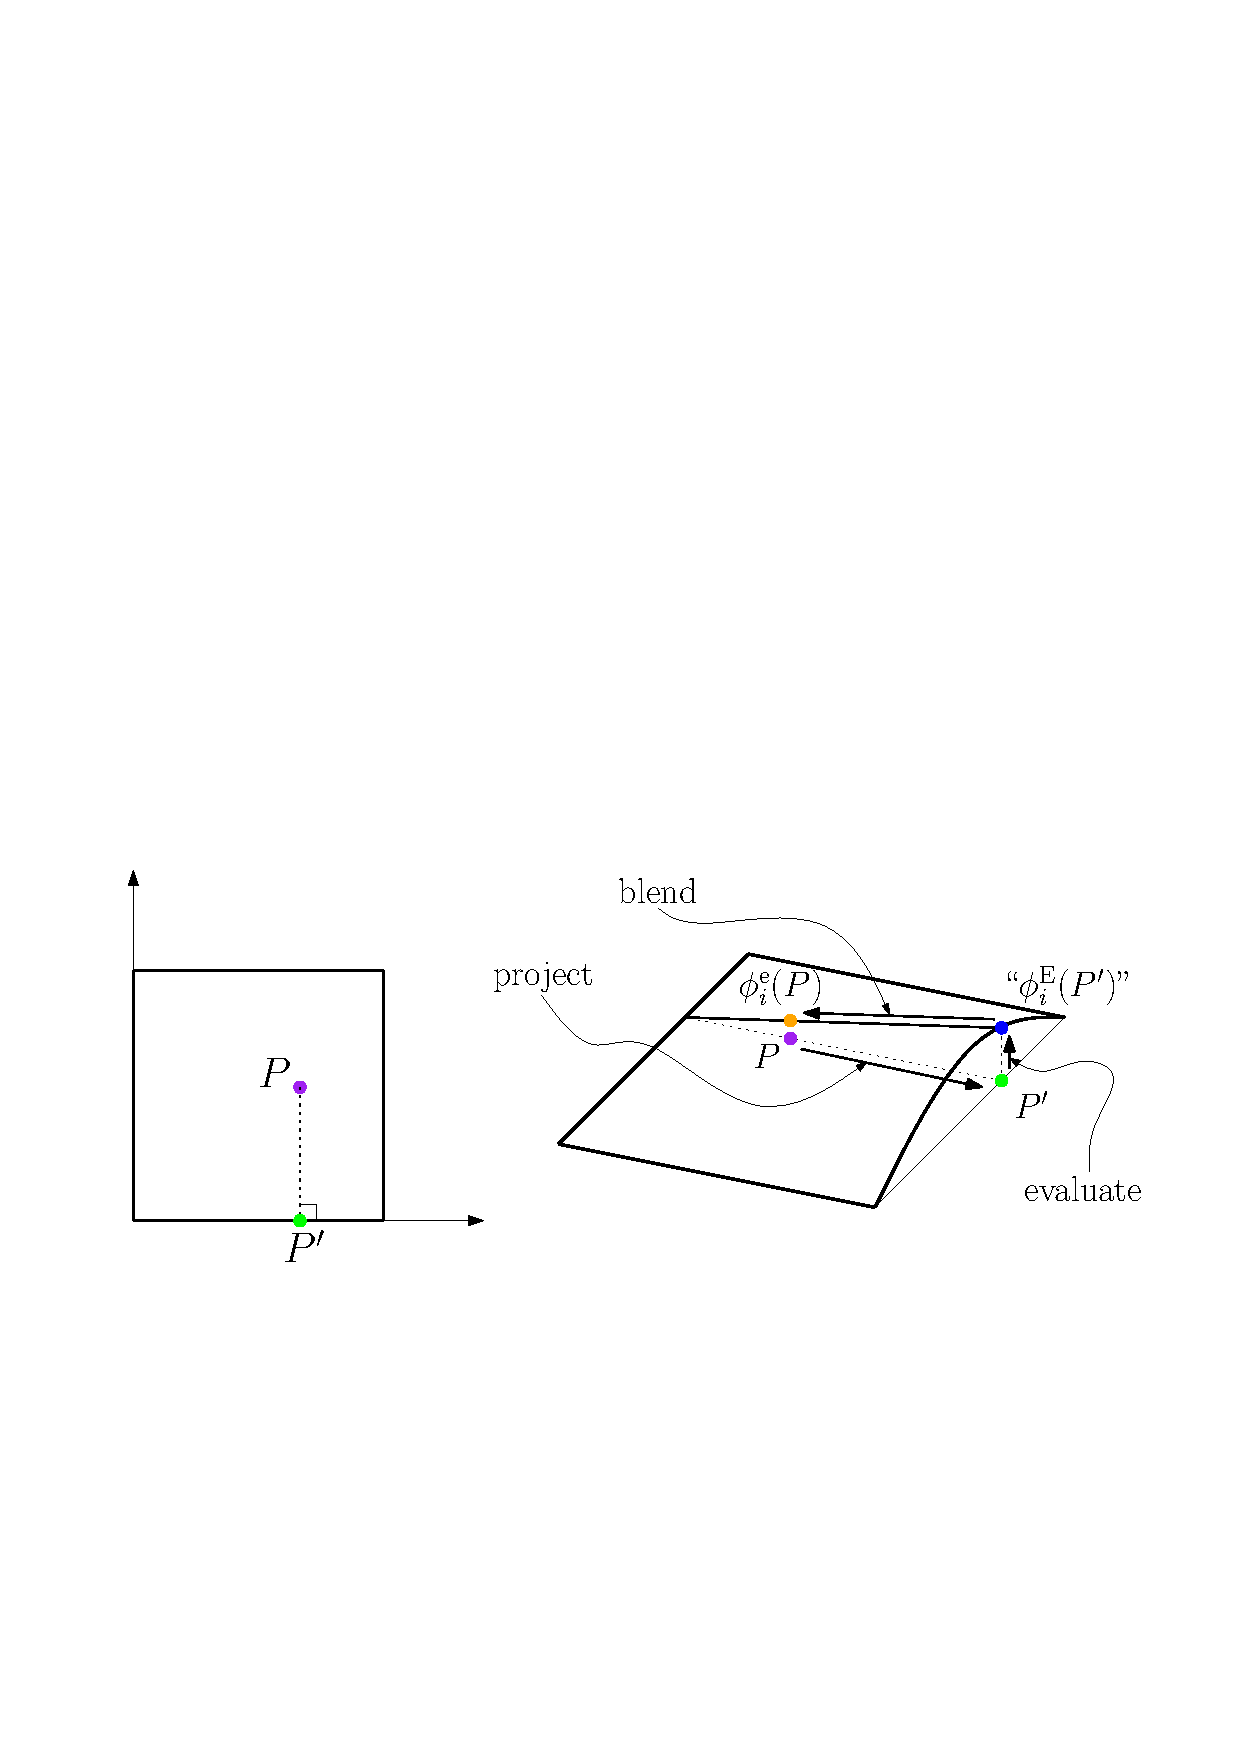
\includegraphics[scale=0.55]{./figures/QuadProjection.pdf}
\caption{Edge projection from $P$ to $P'$, and the logic project$\,\to\,$evaluate$\,\to\,$blend.}
\label{fig:QuadProjection}
\end{center}
\end{figure}

After the original point is projected to the desired edge, it is evaluated at that edge, and finally it is blended linearly:
\begin{equation*}
    \phi_i^\mathrm{e}(\xi)=\underbrace{\mu_0(\xi_2)}_{\text{blend}}
        \underbrace{\phi_i^\E(\underbrace{\vec{\mu}_{01}(\xi_1)}_{\text{project}})}_{\text{evaluate}}
    	=\underbrace{(1-\xi_2)}_{\text{blend}}\underbrace{L_i(\underbrace{\xi_1}_{\text{project}})}_{\text{evaluate}}\,.
\end{equation*}
This blending represents and extension or lifting to the rest of the element.
The whole process of
\begin{equation*}
	\text{projecting}\longrightarrow\text{evaluating}\longrightarrow\text{blending}
\end{equation*}
is extremely important, since it is used in the construction of shape functions for all remaining elements. 
Moreover, as depicted in Figure \ref{fig:QuadProjection}, it gives a geometrical interpretation to the formulas. 
It should be mentioned that if orientations are to be handled, they are taken care of only at the level of evaluating, where a local-to-global transformation will need to be prepended to the original evaluating procedure.
%preprocessing representing a local-to-global transformation will need to be added. 
Projecting and blending are unaffected by orientations.

The general formula for edge functions is
\begin{equation}
    \phi_i^\mathrm{e}(\xi)=\mu_c(\xi_b)\phi_i^\E(\vec{\mu}_{01}(\xi_a))\,,\quad\qquad
    	\nabla\phi_i^\mathrm{e}(\xi)=\mu_c(\xi_b)\nabla\phi_i^\E(\vec{\mu}_{01}(\xi_a))
        +\phi_i^\E(\vec{\mu}_{01}(\xi_a))\nabla\mu_c(\xi_b)\,,\label{eq:QuadH1Edge}
\end{equation}
where $i=2,\ldots,p_a$, $(a,b)=(1,2),(2,1)$ and $c=0,1$, with $p_a$ being the order in the $\xi_a$ coordinate. 
%Their gradients are
%\begin{equation}
%    \nabla\phi_i^\mathrm{e}(\xi)=\mu_c(\xi_b)\nabla\phi_i^\E(\mu_0(\xi_a),\mu_1(\xi_a))
%        +\phi_i^\E(\mu_0(\xi_a),\mu_1(\xi_a))\nabla\mu_c(\xi_b)\,.
%\end{equation}
For example for edge 12 (linked to $\mu_c(\xi_b)=\mu_0(\xi_2)$), this would correspond to $(a,b)=(1,2)$, $c=0$ and $p_a=p$, for edge 23 (linked to $\mu_1(\xi_1)$) it is $(a,b)=(2,1)$, $c=1$ and $p_a=q$, and so on. 
For each edge there are $p_a-1$ shape functions, leading to a total of $2(p-1)+2(q-1)$ edge shape functions.
%Just like 

%\paragraph{Edge Orientations.}
%To consider orientations, simply take a predefined $\oo=0$ orientation, which is determined only by looking at the master element axes and the predefined local edge axes for each edge, and replace $\phi_i^\E$ by $\phi_i^{\e,\oo}$. 
%For example, for edge 12, the local axis $\xi^\mathrm{e}$ is parallel to the master element axis $\xi_1$ and more importantly, it points in the \textit{same} direction. 
%This means the order of the entries in $\phi_i^{\e,\oo}$ is $(\mu_0(\xi_1),\mu_1(\xi_1))$ (and $\textit{not}$ $(\mu_1(\xi_1),\mu_0(\xi_1))$ which would apply if the master element axis and the local axis point in \textit{different} directions). 
%This defines the $\oo=0$ orientation.
%Hence, for edge 12, \eqref{eq:Quadphigeneral} becomes
%\begin{equation*}
%    \phi_i^\mathrm{e}(\xi)\!=\!\mu_0(\xi_2)\phi_i^{\e,\oo}(\mu_0(\xi_1),\mu_1(\xi_1))
%        \!=\!\!\begin{cases}
%            \mu_0(\xi_2)\phi_i^{\e,0}(\mu_0(\xi_1),\mu_1(\xi_1))\!
%            	=\!\mu_0(\xi_2)\phi_i^{\e}(\mu_0(\xi_1),\mu_1(\xi_1))\,\,\,\text{if }\oo=0\\
%            \mu_0(\xi_2)\phi_i^{\e,1}(\mu_0(\xi_1),\mu_1(\xi_1))\!
%            	=\!\mu_0(\xi_2)\phi_i^{\e}(\mu_1(\xi_1),\mu_0(\xi_1))\,\,\,\text{if }\oo=1\,,
%        \end{cases}
%\end{equation*}
%where \eqref{eq:edgeorientations} was used as the definition of $\phi_i^{\e,\oo}$. 
%The same applies to the gradients, and the other edge functions that follow in $H(\mathrm{curl})$ (which involve $E_i^\E$, to be defined later). 
%
%The predefined local edge axis is defined at the master element level.
%These predefined axes for each master element edge are shown in the Appendix.
%The predefined local axis explained above for edge 12 is actually the one utilized in our implementation.
%Naturally, in a different implementation one could decide to use other predefined local edge axes, and the $\oo=0$ orientation would change accordingly as explained above.
%In future examples we will only mention those predefined local edge axes that were used in our implementation (see Appendix).

\subsubsection{\texorpdfstring{$H^1$}{H1} Face Bubbles}

The quadrilateral face bubbles can be naturally defined as the tensor product of 1D edge bubbles,
\begin{equation*}
    \phi_{ij}^\mathrm{f}(\xi)=\phi_i^\E(\vec{\mu}_{01}(\xi_1))\phi_j^\E(\vec{\mu}_{01}(\xi_2))\,,
\end{equation*}
for $i=2,\ldots,p$ and $j=2,\ldots,q$. 
Using \eqref{eq:phiEvanishing}, it is clear the vanishing conditions over all four edges are satisfied.
%For this, note it is used that $\textit{both}$ functions vanish at both endpoints.
This motivates a more general definition.

\begin{definition*}
Let $(s_0,s_1)$ and $(t_0,t_1)$ be two pairs of coordinates which are arbitrary functions of some spatial variable in $\R^N$, $N=2,3$. Let $p_s$ be the order in the $(s_0,s_1)$ coordinates, and $p_t$ be the order in the $(t_0,t_1)$ coordinates. Then
\begin{equation}
    \phi_{ij}^\square(s_0,s_1,t_0,t_1)=\phi_i^\E(s_0,s_1)\phi_j^\E(t_0,t_1)\,,
\end{equation}
for $i=2,\ldots,p_s$ and $j=2,\ldots,p_t$. The gradients, understood in $\R^N$, are
\begin{equation}
	\begin{aligned}
    \nabla\phi_{ij}^\square(s_0,s_1,t_0,t_1)&=\phi_i^\E(s_0,s_1)\nabla\phi_j^\E(t_0,t_1)+\phi_j^\E(t_0,t_1)\nabla\phi_i^\E(s_0,s_1)\,.
	\end{aligned}
\end{equation}
\end{definition*}

%To lighten notation, sometimes the coordinate pair $(s_0,s_1)$ or more technically $(s_0(\bcdot),s_1(\bcdot))$ with $(\bcdot)\in\R^N$, is simply referred to as $\vec{s}(\bcdot)$. Hence, from now on, $\vec{\mu}(\xi_a)=(\mu_0(\xi_a),\mu_1(\xi_a))$ for $a=1,2$.

Rewritten in terms of $\phi_{ij}^\square$, the general formulas for the bubbles and their gradients are,
\begin{equation}
    \phi_{ij}^\mathrm{f}(\xi)=\phi_{ij}^\square(\vec{\mu}_{01}(\xi_1),\vec{\mu}_{01}(\xi_2))\,,\qquad\quad
        \nabla\phi_{ij}^\mathrm{f}(\xi)=\nabla\phi_{ij}^\square(\vec{\mu}_{01}(\xi_1),\vec{\mu}_{01}(\xi_2))\,,
\end{equation}
where $i=2,\ldots,p$ and $j=2,\ldots,q$. 
There are a total of $(p-1)(q-1)$ such functions. 
%They are referred to as \textit{the} 2D $H^1$ quadrilateral face bubbles.

\subsection{\texorpdfstring{$H(\mathrm{curl})$}{Hcurl} Shape Functions}
%As a reminder, in two dimensions, the trace of $H(\mathrm{curl})$ functions is the tangential component of the vector function along the boundary (that is, the edges).
%Hence, all edge functions should have vanishing trace at all other edges, while the bubbles should have zero trace at all edges. 
It will be clear that all shape functions will lie in $\mathcal{Q}^{p-1,q}\times\mathcal{Q}^{p,q-1}$. 
Moreover, after all functions are defined, a rigorous count will give $p(q+1)+(p+1)q$, which is precisely the dimension of $\mathcal{Q}^{p-1,q} \times\mathcal{Q}^{p,q-1}$, so that the shape functions span the desired space.
%That is, the shape functions will span precisely $\mathcal{Q}^{p-1,q} \times\mathcal{Q}^{p,q-1}$, as desired.

\subsubsection{\texorpdfstring{$H(\mathrm{curl})$}{Hcurl} Edges}
\label{sec:HcurledgesQuad}
%To begin to understand what is required of $H(\mathrm{curl})$ edge functions, the first important fact to highlight is that at the level of traces the exact sequence is also satisfied for edges (which are one dimensional segments).
%More precisely, the two dimensional edge functions in $H^1$ should have traces in the on dimensional $H^1(\e)$, while the the two dimensional edge functions in $H(\mathrm{curl})$ should have trace in $L^2(\e)$.
%The following diagram gives a better illustration:
%\begin{displaymath}
%    %\text{2D:}&\qquad H^1 \xrightarrow{\,\,\nabla\,\,} H(\mathrm{curl}) \xrightarrow{\nabla\times} L^2 \\
%    %\text{1D:}&\qquad H^1 \xrightarrow{\,\,\nabla\,\,} L^2\,.
%    \xymatrix{
%        {\text{2D:}} & H^1 \ar[r]^{\nabla\,\,\,\,} \ar[d]^{\mathrm{tr}} & H(\mathrm{curl})
%            \ar[r]^{\,\,\nabla\times} \ar[d]^{\mathrm{tr}} & L^2\\
%        {\text{1D:}} & H^1 \ar[r]^{\nabla\,\,\,\,} & \,\,\,\,L^2\,\, }
%\end{displaymath}
%This should be satisfied at the level of polynomial spaces as well.

First, take for instance edge 12.
As mentioned in \S\ref{sec:dimensionalhierarchy}, the tangential trace of the $H(\mathrm{curl})$ edge functions should be a 1D $L^2$ shape function.
%will take the form of one of \textit{the} 1D $L^2$ edge functions over the tangential trace.
From \eqref{eq:the1DL2edge}, the 1D $L^2$ edge functions (with coordinate $\xi_1$) are $[P_i](\vec{\mu}_{01}(\xi_1))$.
Meanwhile, note the tangential vector to edge 12 is $(1,0)=\nabla\mu_1(\xi_1)$.
When coupled with a blending factor, $\mu_0(\xi_2)$, representing a linear decay (like that of $H^1$), this suggests,
\begin{equation*}
    E_i^\mathrm{e}(\xi)=\mu_0(\xi_2)[P_i](\vec{\mu}_{01}(\xi_1))\nabla\mu_1(\xi_1)
    	=(1-\xi_2)P_i(\xi_1)\Big(\begin{smallmatrix}1\\[2pt]0\end{smallmatrix}\Big)\,,
\end{equation*}
for $i=0,\ldots,p-1$.
%Thus, this $H(\mathrm{curl})$ function has the same linear edge blending across the quadrilateral face as also linear. 
Next, the trace properties are checked.
For this, note that $(0,1)=\nabla\mu_1(\xi_2)$ is the tangent direction to the edges 23 and 14 (where $\xi_1=1$ and $\xi_1=0$ respectively). Hence,
\begin{align*}
    \mathrm{tr}(E_i^\mathrm{e}(\xi))|_{\xi_2=0}&=E_i^\mathrm{e}(\xi)|_{\vec{\mu}_{01}(\xi_2)=(1,0)}\cdot(v_2-v_1)
    		=1\cdot[P_i](\vec{\mu}_{01}(\xi_1))\cdot1=[P_i](\vec{\mu}_{01}(\xi_1))\,,\\
    \mathrm{tr}(E_i^\mathrm{e}(\xi))|_{\xi_1=1}&=E_i^\mathrm{e}(\xi)|_{\vec{\mu}_{01}(\xi_1)=(0,1)}\cdot(v_3-v_2)
    		=\mu_0(\xi_2)[P_i](0,1)\cdot0=0\,,\\
  	\mathrm{tr}(E_i^\mathrm{e}(\xi))|_{\xi_2=1}&=E_i^\mathrm{e}(\xi)|_{\vec{\mu}_{01}(\xi_2)=(0,1)}\cdot(v_3-v_4)
    		=0\cdot[P_i](\vec{\mu}_{01}(\xi_1))\cdot1=0\,,\\
    \mathrm{tr}(E_i^\mathrm{e}(\xi))|_{\xi_1=0}&=E_i^\mathrm{e}(\xi)|_{\vec{\mu}_{01}(\xi_1)=(1,0)}\cdot(v_4-v_1)
    		=\mu_0(\xi_2)[P_i](1,0)\cdot0=0\,.
\end{align*}
The trace properties are then satisfied. Inspired by first order Whitney functions, this motivates the following more general definition.

%Now, consider for example edge 12. Then, the trace of $H^1$ quadrilateral edge functions shown in \eqref{eq:Quadphigeneral} is clearly of the form
%\begin{equation*}
%    \phi_i^\mathrm{e}(\xi)|_{\xi_2=0}=\phi_i^\E(\mu_0(\xi_1),\mu_1(\xi_1))=L_i(\xi_1)\,,
%\end{equation*}
%which, as expected, coincide with the $H^1(\e)$ segment bubble functions shown in \eqref{eq:phiEgeneral}.
%The idea is to have this property for the potential $H(\mathrm{curl})$ edge functions as well.
%Such a function, $E_i^\mathrm{e}(\xi)$, should have edge traces that span the $L^2(\e)$ space for the segment. That is, they should have edge traces like $P_i(\xi_1)$. Since the tangential component of vector function over edge 12 is just its first component, and with a correct blending function to ensure vanishing at the top edge, this leads to:
%\begin{equation*}
%    E_i^\mathrm{e}(\xi)=\mu_0(\xi_2)P_i(\xi_1)\Big(\begin{smallmatrix}1\\[2pt]0\end{smallmatrix}\Big)\,.
%\end{equation*}

\begin{definition*}
Let $s_0$ and $s_1$ be arbitrary functions of some spatial variable in $\R^N$, with $N=2,3$. Denote by $p_s$ the order in the coordinate pair $(s_0,s_1)$. Then
\begin{equation}
    E^\E_i(s_0,s_1)=[P_i](s_0,s_1)(s_0\nabla s_1-s_1\nabla s_0)\,,\label{eq:Hcurledgefunctions}
\end{equation}
for $i=0,\ldots,p_s-1$, and where the gradients are understood in $\R^N$. The curls are
\begin{equation}
    \nabla\times E_i^\E(s_0,s_1)=(i+2)[P_i](s_0,s_1)\nabla s_0\times\nabla s_1\,.\label{eq:curlsEiE}
\end{equation}
\end{definition*}

Here, if $N=2$, the curl and cross product take the form described in \eqref{eq:2Dcurlandcross}. 
Note $E_i^\E$ involves the gradients of its entries, so that it is actually a differential operator assumed to be acting on a functional space (the entries $s_0,s_1$ are \textit{functions}). 
Hence, the use of the term ancillary \textit{operator} is perhaps more appropriate in this case.
The final expression for the curls is nontrivial (see Lemma \ref{lem:curlformula} below). 
Indeed, it is a very powerful result, since at first it is not evident that there should be no partial derivatives of $P_i$ in \eqref{eq:curlsEiE}. 
Fortunately that is the case. 
In fact, it is a requirement, since the $P_i$ are elements of $L^2$, and their derivatives do not exist in general.
The formula follows from the following lemma coupled with the fact that $[P_i](s_0,s_1)$ is a homogeneous polynomial of total order $i$ in $s_0$ and $s_1$.

\begin{lemma}
\label{lem:curlformula}
Let $\psi_i(s_0,s_1)\in\tilde{\mathcal{P}}^i(s_0,s_1)$ be a homogeneous polynomial of total order $i$ in $s_0$ and $s_1$ , where $s_0$ and $s_1$ are arbitrary functions of some spatial variable in $\R^N$, with $N=2,3$. Then
\begin{equation*}
    \nabla\times\Big(\psi_i(s_0,s_1)(s_0\nabla s_1-s_1\nabla s_0)\Big)=(i+2)\psi_i(s_0,s_1)\nabla s_0\times\nabla s_1\,.
\end{equation*}
\end{lemma}
\begin{proof}
Notice that
\begin{align*}
    \nabla\times(s_0\nabla s_1-s_1\nabla s_0)=\nabla s_0\times\nabla s_1+s_0\nabla\times\nabla s_1
        -\nabla s_1\times\nabla s_0-s_1\nabla\times\nabla s_0=2\nabla s_0\times\nabla s_1\,,
\end{align*}
due to $\nabla\times\nabla s_0=\nabla\times\nabla s_1=0$. Now, consider a monomial $s_0^as_1^b$, so that
\begin{align*}
    \nabla\times\Big(s_0^as_1^b(s_0\nabla s_1-s_1\nabla s_0)\Big)
        &=s_0^as_1^b\nabla\times(s_0\nabla s_1-s_1\nabla s_0)+\nabla(s_0^as_1^b)\times(s_0\nabla s_1-s_1\nabla s_0)\\
        &=2s_0^as_1^b\nabla s_0\times\nabla s_1
            +(as_0^{a-1}s_1^b\nabla s_0+bs_0^{a}s_1^{b-1}\nabla s_1)\times(s_0\nabla s_1-s_1\nabla s_0)\\
        &=2s_0^as_1^b\nabla s_0\times\nabla s_1+as_0^{a-1}s_1^bs_0\nabla s_0\times\nabla s_1
            -bs_0^{a}s_1^{b-1}s_1\nabla s_1\times\nabla s_0\\
        &=(2+a+b)s_0^as_1^b\nabla s_0\times\nabla s_1\,,
\end{align*}
where it is used that $\nabla s_0\times \nabla s_0=\nabla s_1\times \nabla s_1=0$. Then observe that any homogeneous polynomial $\psi_i(s_0,s_1)$ is composed of monomials of the form $s_0^as_1^b$ of fixed total order $a+b=i$. The result follows.
\end{proof}

%These are very powerful results, since at first it is not trivial at all that there should be no partial derivatives of $P_i$ in \eqref{eq:curlsEiE}. Fortunately that is the case. In fact, it is a requirement, since the $P_i$ are elements of $L^2$, and their derivative does not exist in general.
Next, record the following important remark.

\begin{remark}
Let $\mu_0=1-\mu_1$, where $\mu_1$ is an arbitrary function of some spatial variable in $\R^N$, with $N=2,3$, and where $p$ is the order in the coordinates $(\mu_0,\mu_1)$. Then for all $i=0,\ldots,p-1$,
\begin{equation}
    E_i^\E(\mu_0,\mu_1)=P_i(\mu_1)\nabla\mu_1\,,\quad\qquad \nabla\times E_i^\E(\mu_0,\mu_1)=0\,.\label{eq:Hcurl1Dspecialcase}
\end{equation}
\end{remark}

With this new ancillary function in our toolset, the $H(\mathrm{curl})$ shape functions for edge 12 are written analogously to those in $H^1$, and the same logic of project$\,\to\,$evaluate$\,\to\,$blend applies,
\begin{equation*}
    E_i^\mathrm{e}(\xi)=\underbrace{\mu_0(\xi_2)}_{\text{blend}}
        \underbrace{E_i^\E(\underbrace{\vec{\mu}_{01}(\xi_1)}_{\text{project}})}_{\text{evaluate}}\,.
\end{equation*}
%Thus, in $H(\mathrm{curl})$ the edge blending across the quadrilateral face is again given by the linear function $\mu_0(\xi_2)$. 

In general, the edge shape functions and their curls are
\begin{equation}
    E_i^\mathrm{e}(\xi)=\mu_c(\xi_b)E_i^\E(\vec{\mu}_{01}(\xi_a))\,,\qquad\quad
    \nabla\times E_i^\mathrm{e}(\xi)=\nabla\mu_c(\xi_b)\times E_i^\E(\vec{\mu}_{01}(\xi_a))\,,
    \label{eq:QuadHcurlEdge}
\end{equation}
where $i=0,\ldots,p_a-1$, $(a,b)=(1,2),(2,1)$ and $c=0,1$. There are $p_a$ functions for each edge, giving a total of $2p+2q$ edge shape functions.

\subsubsection{\texorpdfstring{$H(\mathrm{curl})$}{Hcurl} Face Bubbles}

In general, the idea is to consider the tensor product of the ancillary functions $E_i^\E$ and $\phi_j^\E$, evaluated at the 1D affine coordinate pairs $\vec{\mu}_{01}(\xi_1)$ and $\vec{\mu}_{01}(\xi_2)$. 
To cover all possibilities, one must consider both $\phi_j^\E(\vec{\mu}_{01}(\xi_2))E_i^\E(\vec{\mu}_{01}(\xi_1))$ and $\phi_j^\E(\vec{\mu}_{01}(\xi_1))E_i^\E(\vec{\mu}_{01}(\xi_2))$.
Clearly, both of these cases are actually generated by a single key operator $E_{ij}^\square$, which is defined generally next.

\begin{definition*}
Let $(s_0,s_1)$ and $(t_0,t_1)$ be two pairs of coordinates which are arbitrary functions of some spatial variable in $\R^N$, with $N=2,3$. Let $p_s$ be the order in the $(s_0,s_1)$ coordinates, and $p_t$ be the order in the $(t_0,t_1)$ coordinates. Then
\begin{equation}
    E_{ij}^{\square}(s_0,s_1,t_0,t_1)=\phi_j^\E(t_0,t_1)E_i^\E(s_0,s_1)\,,
\end{equation}
for $i=0,\ldots,p_s-1$ and $j=2,\ldots,p_t$. The curls, understood in $\R^N$, are
\begin{equation}
    \nabla\times E_{ij}^{\square}(s_0,s_1,t_0,t_1)=\phi_j^\E(t_0,t_1)\nabla\times E_i^\E(s_0,s_1)
    	+\nabla\phi_j^\E(t_0,t_1)\times E_i^\E(s_0,s_1)\,.
\end{equation}
%Also
%\begin{equation}
%    E_{ij}^{\square_{II}}(s_0,s_1,t_0,t_1)=\phi_i^\E(s_0,s_1)E_j^\E(t_0,t_1),
%\end{equation}
%for $i=2,\ldots,p_s$ and $j=0,\ldots,p_t-1$. The curls are
%\begin{equation}
%    \nabla\times E_{ij}^{\square_{II}}(s_0,s_1,t_0,t_1)=\phi_i^\E(t_0,t_1)\nabla\times E_j^\E(t_0,t_1)
%    +\nabla\phi_i^\E(s_0,s_1)\times E_j^\E(t_0,t_1)\,.
%\end{equation}
\end{definition*}
%Record also the useful result
%\begin{remark}
%If $\mu_0^(1)=1-\mu_1^(1)$ and $\mu_0^(2)=1-\mu_1^(2)$, where $\mu_1^(1)$ and $\mu_1^(2)$ are arbitrary functions of some spatial variable in $\R^N$ with $N=2,3$, then
%\begin{equation}
%   E_{ij}^{\square_I}(\mu_0^(1),\mu_1^(1),\mu_0^(2),\mu_1^(2))=L_j(\mu_1^(2))P_i(\mu_1^(1))\nabla\mu_1^(1)\,,\qquad\nabla\times
%   E_i^\E(\mu_0,\mu_1)=P_i(\mu_1)\nabla\mu_1\,,\quad\qquad \nabla\times E_i^\E(\mu_0,\mu_1)=0\,.
%\end{equation}
%\end{remark}
Using \eqref{eq:phiEvanishing}, and proceeding as with the $H(\mathrm{curl})$ edge functions, it is clear that this ancillary operator, when evaluated at  $(\vec{\mu}_{01}(\xi_1),\vec{\mu}_{01}(\xi_2))$ or  $(\vec{\mu}_{01}(\xi_2),\vec{\mu}_{01}(\xi_1))$, satisfies the necessary vanishing trace at all edges. 
There are two families, which together comprise $p(q-1)+q(p-1)$ bubble functions.
%As a group, they are referred to as \textit{the} 2D $H(\mathrm{curl})$ quadrilateral face bubbles.

\subparagraph{Family I:}
The shape functions for the first family and their corresponding curls are
\begin{equation}
    E_{ij}^{\mathrm{f}}(\xi)=E_{ij}^{\square}(\vec{\mu}_{01}(\xi_1),\vec{\mu}_{01}(\xi_2))\,,\qquad
    \nabla\times E_{ij}^{\mathrm{f}}(\xi)=\nabla\times E_{ij}^{\square}(\vec{\mu}_{01}(\xi_1),\vec{\mu}_{01}(\xi_2))\,,
\end{equation}
for $i=0,\ldots,p-1$ and $j=2,\ldots,q$.
There are $p(q-1)$ shape functions in this family.

\subparagraph{Family II:}
The shape functions for the second family and their corresponding curls are
\begin{equation}
    E_{ij}^{\mathrm{f}}(\xi)=E_{ij}^{\square}(\vec{\mu}_{01}(\xi_2),\vec{\mu}_{01}(\xi_1))\,,\qquad
    \nabla\times E_{ij}^{\mathrm{f}}(\xi)=\nabla\times E_{ij}^{\square}(\vec{\mu}_{01}(\xi_2),\vec{\mu}_{01}(\xi_1))\,,
\end{equation}
for $i=0,\ldots,q-1$ and $j=2,\ldots,p$. 
Notice the only difference with the first family is that the entries $\vec{\mu}_{01}(\xi_1)$ and $\vec{\mu}_{01}(\xi_2)$ are permuted (along with the associated orders $p$ and $q$).
%This has the effect that internally within $E_{ij}^{\square}$, $E_i^\E$ and $\phi_j^\E$ are now related to the $\vec{\mu}_{01}(\xi_2)$ and $\vec{\mu}_{01}(\xi_1)$ respectively and as a result there are $q(p-1)$ shape functions in this family.
Hence, there are $q(p-1)$ shape functions in this family.

\subsection{\texorpdfstring{$H(\mathrm{div})$}{Hdiv} Shape Functions}

By the definition of the $H(\mathrm{div})$ space (see \eqref{eq:Hdiv2Ddef}) in two dimensions, it is clear that it is isomorphic to $H(\mathrm{curl})$. 
Indeed, the $H(\mathrm{div})$ shape functions will be the rotation of the corresponding $H(\mathrm{curl})$ shape functions. 
More explicitly, given a shape function $E\in H(\mathrm{curl})$ and its curl $\nabla\times E\in L^2$, the corresponding $H(\mathrm{div})$ shape function with its divergence is
\begin{equation}
    V=\begin{pmatrix}0&1\\-1&0\end{pmatrix}E\,,\quad\qquad\nabla\cdot V=\nabla\times E\,.
\end{equation}
Note in this case the original polynomial space $Q^{p,q}=\mathcal{Q}^{p-1,q}\times\mathcal{Q}^{p,q-1}$ for $H(\mathrm{curl})$ simply becomes the $H(\mathrm{div})$ conforming space $V^{p,q}=\mathcal{Q}^{p,q-1}\times\mathcal{Q}^{p-1,q}$.


\subsection{\texorpdfstring{$L^2$}{L2} Shape Functions}

%These should span the same space as the span of the curls of the $H(\textrm{curl})$ shape functions.
As expected, they are the tensor products of the 1D $L^2$ shape functions, and there are $pq$ such functions spanning $\mathcal{Q}^{p-1,q-1}$.

\subsubsection{\texorpdfstring{$L^2$}{L2} Face}

The coordinate free $L^2$ shape functions for the quadrilateral faces are
\begin{equation}
    \psi_{ij}^\mathrm{f}(\xi)=P_i(\mu_1(\xi_1))P_j(\mu_1(\xi_2))
    	=[P_i](\vec{\mu}_{01}(\xi_1))[P_j](\vec{\mu}_{01}(\xi_2))(\nabla\mu_1(\xi_1)\!\!\times\!\!\nabla\mu_1(\xi_2))\,,
   \label{eq:QuadL2Functions}
\end{equation}
for $i=0,\ldots,p-1$ and $j=0,\ldots,q-1$. There are $pq$ face functions. 
The factor $\nabla\mu_1(\xi_1)\!\times\!\nabla\mu_1(\xi_2)$ makes the expression coordinate free (with the $\xi$ coordinates it is $1$).

\subsection{Orientations}
\label{sec:QuadOrientations}

For 2D quadrilaterals, only edge orientations need to be considered to ensure compatibility.
However, in 3D elements, quadrilateral \textit{faces} will have the notion of orientation, and one will need to consider this to ensure full compatibility.
In view of this, first we will show how the concept of edge orientations, already explained in \S\ref{sec:edgeorientations}, applies to the quadrilateral element. We assume that section has been covered.
After that, the quadrilateral face orientations are introduced as a preview to the 3D elements.

\subsubsection{Edge Orientations}
\label{sec:QuadEdgeOrientations}

\begin{figure}[!ht]
\begin{center}
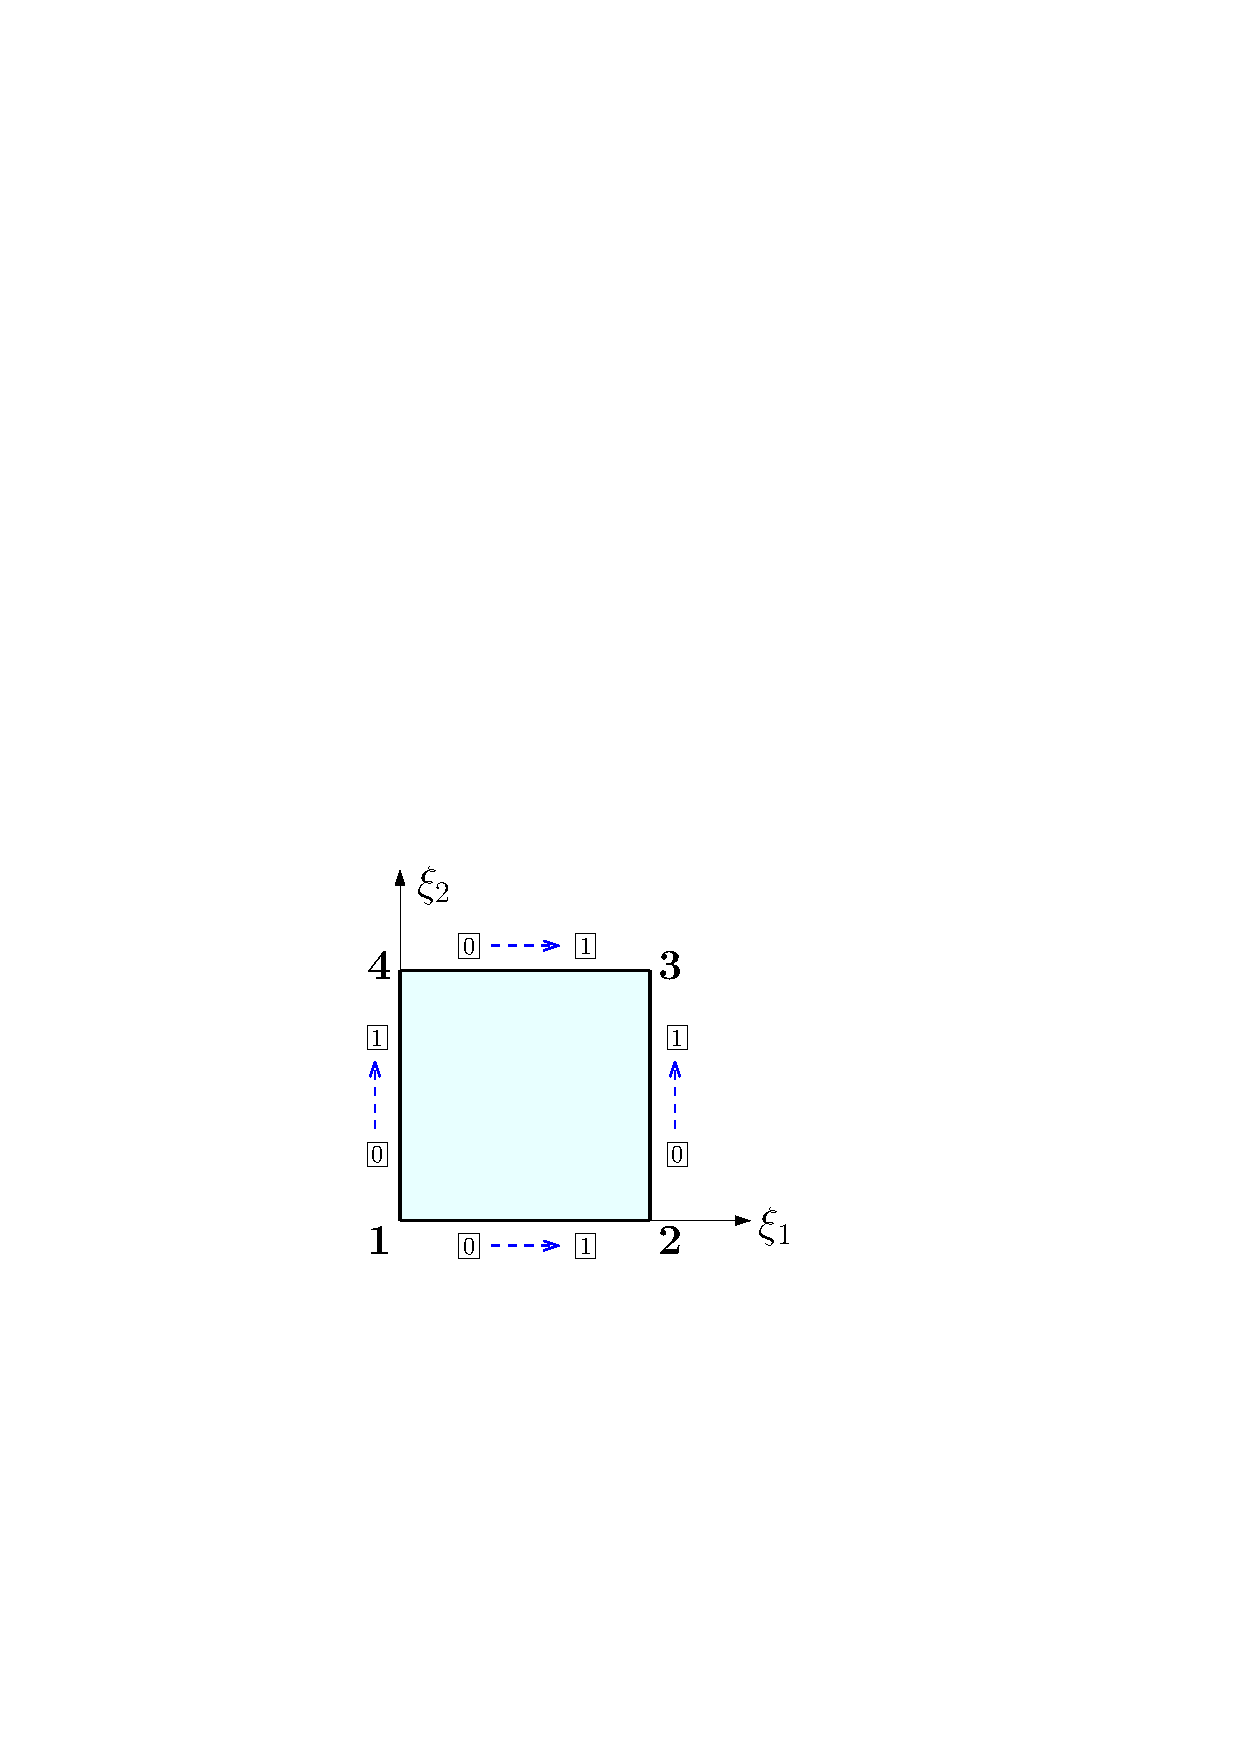
\includegraphics[scale=0.5]{./figures/MasterQuadOrientations.pdf}
\caption{Master quadrilateral with local edge orientations.}
\label{fig:MasterQuadOrientations}
\end{center}
\end{figure}

The master quadrilateral has a predefined \textit{local} orientation for each edge, which reperesents the $\oo=0$ case. 
These are illustrated in Figure \ref{fig:MasterQuadOrientations}.
They are \textit{our} choices for the local orientations.

%Recall each vertex has its own pair of 1D coordinates associated to it in the expression for the vertex functions (see \S\ref{sec:H1QuadVertices}). 
%That is, the vertex with coordinates $(a,b)$ is associated to the coordinates $\mu_a(\xi_1)$ and $\mu_b(\xi_2)$. %, while vertex 2 is associated to $\mu_1(\xi_1)$ and $\mu_0(\xi_2)$, and so on.
%When analizing a given edge, each of its two vertices have two 1D affine coordinates associated to them (so there is a total of four). Two of these will match and the other two will differ. 
%For example, for edge 12, with vertices 1 and 2, the coordinate $\mu_0(\xi_2)$ is shared by both vertices, but the coordinates $\mu_0(\xi_1)$ (related to vertex 1) and $\mu_1(\xi_1)$ (related to vertex 2) differ.
%The order in which these different coordinates are specified determines the $\oo=0$ local orientation.
%In edge 12, the local axis points from vertex 1 to vertex 2, so that the order of the coordinates should be $\mu_0(\xi_1)$ (related to vertex 1) followed by $\mu_1(\xi_1)$ (related to vertex 2).
Each edge has a local orientation described by the fixed ordering $\boxednum{0}\!\tdashto\boxednum{1}$.
This induces a master element \textit{local} edge vertex-ordering, which in turn determines a \textit{locally ordered} pair of affine coordinates, since, over a given edge, each master element vertex is linked to one affine coordinate.
For instance, over edge 12, $v_1$ is linked to $\mu_0(\xi_1)$ and $v_2$ linked to $\mu_1(\xi_1)$.
On this edge the induced master element \textit{local} ordering is $v_1\tdashto v_2$ (see Figure \ref{fig:MasterQuadOrientations}), meaning that the locally ordered pair is $\vec{\mu}_{01}(\xi_1)=(\mu_0(\xi_1),\mu_1(\xi_1))$.
The locally ordered pair represents the local coordinates, and it serves as the input of the edge local-to-global transformation $\sigma_\oo^\E$, which transforms them to a globally ordered pair (depending on the parameter $\oo$).
The globally ordered pair is then introduced into the edge ancillary functions of the edge shape functions, and the resulting functions are said to be \textit{orientation embedded} shape functions.
Thus, for example for edge 12 the orientation embedded $H^1$ edge functions are, 
\begin{equation*}
    \phi_i^\mathrm{e}(\xi)=\mu_0(\xi_2)\phi_i^\E\circ\sigma_\oo^\E(\vec{\mu}_{01}(\xi_1))
        =\begin{cases}
            \mu_0(\xi_2)\phi_i^\E\Big(\sigma_0^\E(\vec{\mu}_{01}(\xi_1))\Big)
            	=\mu_0(\xi_2)\phi_i^\E(\mu_0(\xi_1),\mu_1(\xi_1))\,\,\,\text{if }\oo=0\,,\\
            \mu_0(\xi_2)\phi_i^\E\Big(\sigma_1^\E(\vec{\mu}_{01}(\xi_1))\Big)
            	=\mu_0(\xi_2)\phi_i^{\e}(\mu_1(\xi_1),\mu_0(\xi_1))\,\,\,\text{if }\oo=1\,,
        \end{cases}
\end{equation*}
for $i=2,\ldots,p$.
This composition with $\sigma_\oo^\E$ naturally applies to all 2D edge functions in $H^1$ and $H(\mathrm{curl})$ and their differential forms. 
Hence, $\sigma_\oo^\E$ should be composed with $\phi_i^\E$, $\nabla\phi_i^\E$, $E_i^\E$ and $\nabla\times E_i^\E$ in \eqref{eq:QuadH1Edge} and \eqref{eq:QuadHcurlEdge}.


%Over each edge there is always a 1D affine coordinate duple $\vec{\mu}_{01}(\xi_a)=(\mu_0(\xi_a),\mu_1(\xi_a))$ for some $a=1,2$ which  induces a projection as described in \S\ref{sec:H1edgesQuad}.
%In fact, each affine coordinate is linked to a vertex of the edge being analyzed.
%For instance, in edge 12, $v_1$ is linked to $\mu_0(\xi_1)$, while $v_2$ is linked to $\mu_1(\xi_1)$.
%Now, the edge in question has a fixed local orientation described by a fixed local ordering $\boxednum{0}\!\tdashto\boxednum{1}$, which in turn induces a master element \textit{local} edge vertex-ordering.
%For edge 12, the master element \textit{local} edge vertex-ordering is $v_1\tdashto v_2$ (see Figure \ref{fig:MasterQuadOrientations}).
%This then generates an ordering of the affine coordinates, where first comes $\mu_0(\xi_1)$ linked to $v_1$ followed by $\mu_1(\xi_1)$ linked to $v_2$, so that the ordered affine coordinates are $\vec{\mu}_{01}(\xi_1)=(\mu_0(\xi_1),\mu_1(\xi_1))$ (as opposed to $\vec{\mu}_{10}(\xi_1)=(\mu_1(\xi_1),\mu_0(\xi_1))$ if $v_2\to v_1$).
%In this case, the affine coordinates are said to be \textit{locally ordered}, and in this form, they serve as the input for the edge orientation permutation function $\sigma_\oo^\E$.
%Indeed, the locally ordered affine coordinates represent the local $\oo=0$ orientation.
%%Note that the other alternative was that the master element ordering would have been 
%%Hence the \textit{ordered} pair of coordinates is $\vec{\mu}_{01}(\xi_1)=(\mu_0(\xi_1),\mu_1(\xi_1))$, as opposed to $\vec{\mu}_{10}(\xi_1)=(\mu_1(\xi_1),\mu_0(\xi_1))$.
%%The locally ordered
%The ancillary functions are then modified as described in \S\ref{sec:edgeorientations}, by composing first with $\sigma_\oo^\E$, which represents a local-to-global transformation.
%These modified functions are then replaced in the expressions of the shape functions to produce the \textit{orientation embedded} shape functions.
%Thus, for example for edge 12 the orientation embedded $H^1$ edge functions are, 
%\begin{equation*}
%    \phi_i^\mathrm{e}(\xi)=\mu_0(\xi_2)\phi_i^\E\circ\sigma_\oo^\E(\vec{\mu}_{01}(\xi_1))
%        =\begin{cases}
%            \mu_0(\xi_2)\phi_i^\E\Big(\sigma_0^\E(\vec{\mu}_{01}(\xi_1))\Big)
%            	=\mu_0(\xi_2)\phi_i^\E(\mu_0(\xi_1),\mu_1(\xi_1))\,\,\,\text{if }\oo=0\,,\\
%            \mu_0(\xi_2)\phi_i^\E\Big(\sigma_1^\E(\vec{\mu}_{01}(\xi_1))\Big)
%            	=\mu_0(\xi_2)\phi_i^{\e}(\mu_1(\xi_1),\mu_0(\xi_1))\,\,\,\text{if }\oo=1\,,
%        \end{cases}
%\end{equation*}
%for $i=2,\ldots,p$.
%Note that $\sigma_\oo^\E(\vec{\mu}_{01}(\xi_1))\neq\sigma_\oo^\E(\vec{\mu}_{10}(\xi_1))$, so, to be consistent with the local orientations, it is important that $\sigma_\oo^\E$ evaluates specifically the \textit{locally ordered} affine coordinates $\vec{\mu}_{01}(\xi_1)$.  
%These modifications naturally apply also to all 2D expressions involving $\nabla\phi_i^\E$, $E_i^\E$ and $\nabla\times E_i^\E$.
%%Clearly, the projection (as described in \S\ref{sec:H1edgesQuad}) and blending (given by $\mu_0(\xi_2)$) are unaffected by orientations.

\begin{figure}[!ht]
\begin{center}
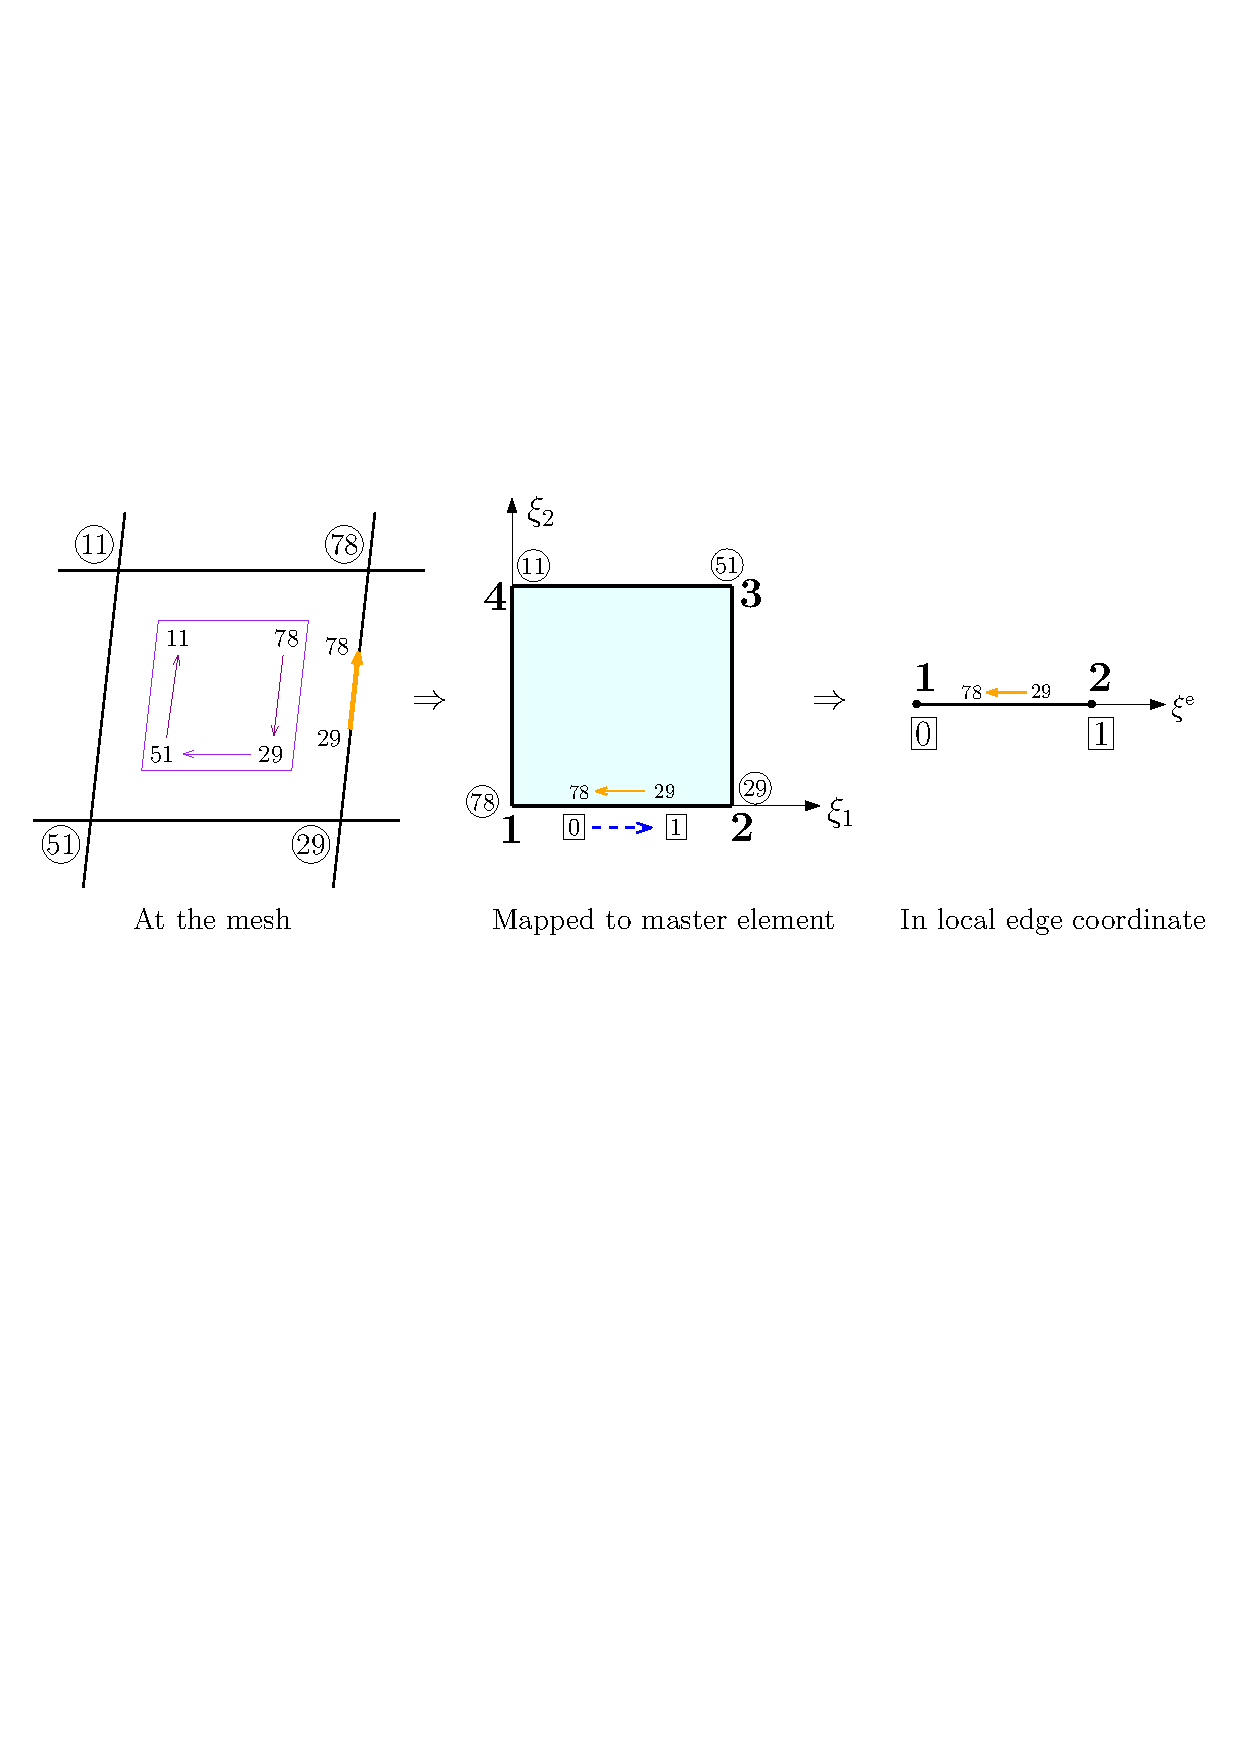
\includegraphics[scale=0.75]{./figures/QuadEdgeOrientExample.pdf}
\caption{A mesh with global edge orientations followed by transformations to master element and local edge coordinates.}
\label{fig:QuadEdgeOrientExample}
\end{center}
\end{figure}

Now, to see a more explicit example starting from the global mesh, consider Figure \ref{fig:QuadEdgeOrientExample}.
There, one can observe a quadrilateral in a mesh with vertices $11$, $29$, $51$ and $78$.
In 2D, Szabo's approach (implicitly) involves specifying a \textit{face vertex-ordering} at the mesh that determines the mapping to the master element, which has a fixed master element ordering $v_1\tto v_2\tto v_3\tto v_4$.
However, there is no independent edge vertex-ordering of each edge.
In this case, the face vertex-ordering at the mesh is shown to be $78\tto29\tto51\tto11$, and at the master element level it coincides with $v_1\tto v_2\tto v_3\tto v_4$.
%This is then mapped to the master element such that it coincides with the fixed master element ordering .
The novelty here is that additionally the mesh edge with vertices $78$ and $29$ also has a \textit{global} orientation given by the edge vertex-ordering $29\tto78$.
This edge is mapped to the master element edge 12 (as induced by the face vertex-ordering), and receives the induced master element \textit{global} ordering $v_2\tto v_1$. 
Clearly, the \textit{local} orientation, given by the induced \textit{local} ordering $v_1\tdashto v_2$, does not coincide with the \textit{global} orientation, meaning that the orientation parameter is $\oo=1$ for this master element edge.
Therefore, the orientation embedded $H^1$ edge shape functions would specifically be,
\begin{equation*}
    \phi_i^\mathrm{e}(\xi)=\mu_0(\xi_2)\phi_i^{\e}\circ\sigma_\oo^\E(\vec{\mu}_{01}(\xi_1))
            	=\mu_0(\xi_2)\phi_i^\E(\mu_1(\xi_1),\mu_0(\xi_1))\,,
\end{equation*}
for $i=2,\ldots,p$. 
The neighboring element in the mesh (also sharing vertices $29$ and $78$) might have a different face vertex-ordering, but it has the \textit{same} edge vertex-ordering at the mesh (the global orientation). 
This can result in another orientation parameter at the master element edge of the neighboring element, but by construction, the fact remains that when mapped back to the global mesh, the shape functions will be fully compatible along that shared edge.  
%For 2D quadrilaterals only edge orientations need to be considered to ensure compatibility.

%\paragraph{Edge Orientations.}
%To consider orientations, simply take a predefined $\oo=0$ orientation, which is determined only by looking at the master element axes and the predefined local edge axes for each edge, and replace $\phi_i^\E$ by $\phi_i^{\e,\oo}$. 
%For example, for edge 12, the local axis $\xi^\mathrm{e}$ is parallel to the master element axis $\xi_1$ and more importantly, it points in the \textit{same} direction. 
%This means the order of the entries in $\phi_i^{\e,\oo}$ is $(\mu_0(\xi_1),\mu_1(\xi_1))$ (and $\textit{not}$ $(\mu_1(\xi_1),\mu_0(\xi_1))$ which would apply if the master element axis and the local axis point in \textit{different} directions). 
%This defines the $\oo=0$ orientation.
%Hence, for edge 12, \eqref{eq:Quadphigeneral} becomes
%\begin{equation*}
%    \phi_i^\mathrm{e}(\xi)\!=\!\mu_0(\xi_2)\phi_i^{\e,\oo}(\mu_0(\xi_1),\mu_1(\xi_1))
%        \!=\!\!\begin{cases}
%            \mu_0(\xi_2)\phi_i^{\e,0}(\mu_0(\xi_1),\mu_1(\xi_1))\!
%            	=\!\mu_0(\xi_2)\phi_i^{\e}(\mu_0(\xi_1),\mu_1(\xi_1))\,\,\,\text{if }\oo=0\\
%            \mu_0(\xi_2)\phi_i^{\e,1}(\mu_0(\xi_1),\mu_1(\xi_1))\!
%            	=\!\mu_0(\xi_2)\phi_i^{\e}(\mu_1(\xi_1),\mu_0(\xi_1))\,\,\,\text{if }\oo=1\,,
%        \end{cases}
%\end{equation*}
%where \eqref{eq:edgeorientations} was used as the definition of $\phi_i^{\e,\oo}$. 
%The same applies to the gradients, and the other edge functions that follow in $H(\mathrm{curl})$ (which involve $E_i^\E$, to be defined later). 
%
%The predefined local edge axis is defined at the master element level.
%These predefined axes for each master element edge are shown in the Appendix.
%The predefined local axis explained above for edge 12 is actually the one utilized in our implementation.
%Naturally, in a different implementation one could decide to use other predefined local edge axes, and the $\oo=0$ orientation would change accordingly as explained above.
%In future examples we will only mention those predefined local edge axes that were used in our implementation (see Appendix).

\subsubsection{Quadrilateral Face Orientations Explained}
\label{sec:QuadFaceOrientations}

\begin{figure}[!ht]
\begin{center}
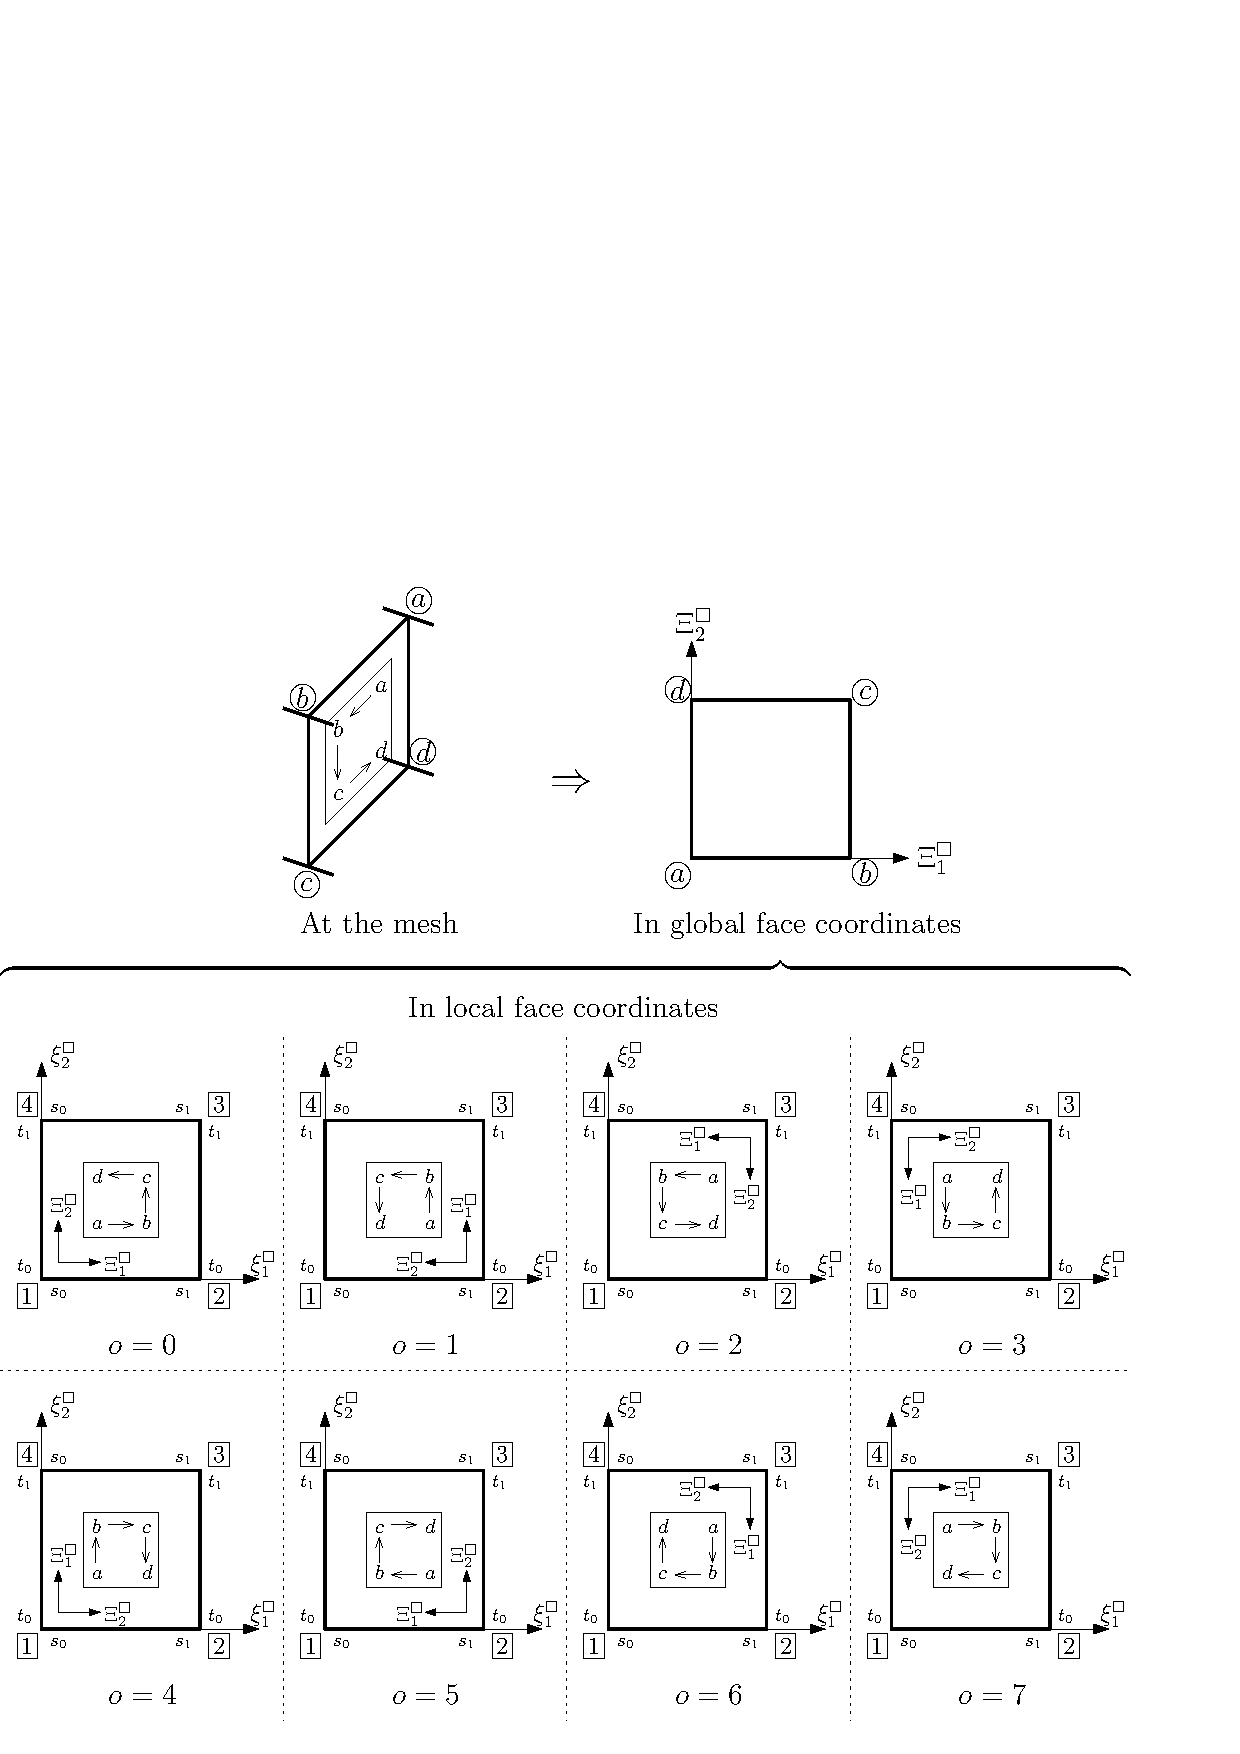
\includegraphics[scale=0.75]{./figures/OrientationsQuad.pdf}
\caption{Quadrilateral face orientations.}
\label{fig:orientationsquad}
\end{center}
\end{figure}

%For quadrilaterals it is not important to consider face orientations, since the boundary, which is shared with adjacent elements, is one dimensional.
%This means only edge orientations need to be considered.
%However, in three dimensions, the boundary is two dimensional.
%This means quadrilateral faces will be shared by adjacent elements.
%It is required to match the corresponding shape functions over these faces to satisfy the compatibility condition.
In 3D, as with edge orientations, each face at the mesh must be given its own \textit{global face orientation} to ensure full compatibility across the boundaries.
For quadrilaterals, this is represented by the global quadrilateral face coordinates $\Xi^\square=(\Xi_1^\square,\Xi_2^\square)$, or equivalently, by the \textit{global face vertex-ordering}.
For example, given a quadrilateral face in the mesh, a vertex-ordering of the form $a\tto b\tto c\tto d$ means the origin of $\Xi^\square$ is located at $a$, $\Xi_1^\square$ points from $a$ to $b$, and $\Xi_2^\square$ points from $a$ to $d$.
Meanwhile, at the master element, the mapped face has its own fixed \textit{local orientation}.
It is represented by the coordinates $\xi^\square=(\xi_1^\square,\xi_2^\square)$ or equivalently by the fixed \textit{local} ordering of the form $\boxednum{1}\!\tdashto\boxednum{2}\!\tdashto\boxednum{3}\!\tdashto\boxednum{4}$.
In general, the two systems of coordinates will not match, and this mismatch is represented by the orientation parameter $\oo$.
In fact, there are \textit{eight} possible orientations for quadrilateral faces, meaning $\oo=0,\ldots,7$.
These are all illustrated in Figure \ref{fig:orientationsquad}.


%Again, as with edge orientations, this will be done by embedding global face coordinate axes to each face in the mesh.
%These are denoted by $\Xi^\mathrm{f}=(\Xi_1^\mathrm{f},\Xi_2^\mathrm{f})$.
%Meanwhile at the master element level, each face (and edge) has a predefined local face (and edge) axis.
%For the faces, these local coordinates are denoted by $\xi^\mathrm{f}=(\xi_1^\mathrm{f},\xi_2^\mathrm{f})$.
%At the master element and given a face, it is clear that the predefined local face axis and the global face axis might not be the same.
%In fact, the main difficulty for the quadrilateral is that there are \textit{eight} possible orientations for each face.
%These are illustrated in Fig.~(\textit{add Figure}).
%They are referred to by the parameter $\oo$ which for quadrilateral faces goes from $0$ to $7$.

As with edges, the idea is to have a local-to-global transformation which depends on the orientation parameter $\oo$.
Here, the \textit{local} orientation is represented by the \textit{locally ordered} quadruple $(s_0,s_1,t_0,t_1)$ composed of the two pairs $(s_0,s_1)$ and $(t_0,t_1)$.
The \textit{first} pair, $(s_0,s_1)$, is a locally ordered pair corresponding to the \textit{first} local face coordinate $\xi_1^\square$ (which as an \textit{edge} coordinate has the local ordering $\boxednum{1}\!\tdashto\boxednum{2}$ or $\boxednum{4}\!\tdashto\boxednum{3}$).
The \textit{second} pair, $(t_0,t_1)$, is a locally ordered pair corresponding to the \textit{second} local face coordinate $\xi_2^\square$ (which as an \textit{edge} coordinate has the local ordering $\boxednum{1}\!\tdashto\boxednum{4}$ or $\boxednum{2}\!\tdashto\boxednum{3}$).
Meanwhile, the \textit{global} orientation is analogously represented by a \textit{globally ordered} quadruple composed of two pairs.
The first pair is a globally ordered pair corresponding to the first global face coordinate $\Xi_1^\square$, and similarly with the second pair.
For example, looking at Figure \ref{fig:orientationsquad}, when $\oo=1$, $\Xi_1^\square$ is associated to $(t_0,t_1)$, while $\Xi_2^\square$ is associated to $(s_1,s_0)$, so that the globally ordered quadruple is $(t_0,t_1,s_1,s_0)$.
This way, the local-to-global transformation is actually a permutation dependent on $\oo$ that can easily be determined by looking at Figure \ref{fig:orientationsquad}.
%As an example consider $\oo=1$, where $\Xi_1^\square$ is associated to the globally ordered pair $(t_0,t_1)$ (via $\boxednum{2}\!\tto\boxednum{3}$ or $\boxednum{1}\!\tto\boxednum{4}$), while $\Xi_2^\square$ is associated to $(s_1,s_0)$ (via $\boxednum{3}\!\tto\boxednum{4}$ or $\boxednum{2}\!\tto\boxednum{1}$).
%Therefore, the globally ordered quadruple is $(t_0,t_1,s_1,s_0)$.
%The full local-to-global transformation is described by the following permutation function. 

\begin{definition*}
Let $s_0$, $s_1$, $t_0$ and $t_1$ be arbitrary variables, and let $\oo=0,1,2,3,4,5,6,7$ be the quadrilateral face orientation parameter. 
The quadrilateral face orientation permutation function, $\sigma_\oo^\square$, is defined as
\begin{equation}
	\sigma_\oo^\square(s_0,s_1,t_0,t_1)=\begin{cases}
		\sigma_0^\square(s_0,s_1,t_0,t_1)=(s_0,s_1,t_0,t_1)&\quad\text{if  }\,\oo=0\,,\\
		\sigma_1^\square(s_0,s_1,t_0,t_1)=(t_0,t_1,s_1,s_0)&\quad\text{if  }\,\oo=1\,,\\
		\sigma_2^\square(s_0,s_1,t_0,t_1)=(s_1,s_0,t_1,t_0)&\quad\text{if  }\,\oo=2\,,\\
		\sigma_3^\square(s_0,s_1,t_0,t_1)=(t_1,t_0,s_0,s_1)&\quad\text{if  }\,\oo=3\,,\\
		\sigma_4^\square(s_0,s_1,t_0,t_1)=(t_0,t_1,s_0,s_1)&\quad\text{if  }\,\oo=4\,,\\
		\sigma_5^\square(s_0,s_1,t_0,t_1)=(s_1,s_0,t_0,t_1)&\quad\text{if  }\,\oo=5\,,\\
		\sigma_6^\square(s_0,s_1,t_0,t_1)=(t_1,t_0,s_1,s_0)&\quad\text{if  }\,\oo=6\,,\\
		\sigma_7^\square(s_0,s_1,t_0,t_1)=(s_0,s_1,t_1,t_0)&\quad\text{if  }\,\oo=7\,.\end{cases}\label{eq:orientQuadFace}
\end{equation}
\end{definition*}

%Clearly, ``outer'' permutations (of the pairs) occur when the global edge axis $\Xi_1^\square$ is parallel to $\xi_2^\square$ (or equivalently if $\Xi_2^\square$ is parallel to $\xi_1^\square$).
%In this case, the axes are said to be \textit{swapped}.
%On the other hand, inner permutations represent the alignment of the parallel axes.
%If inner permutations are applied \textit{after} outer permutations, then the inner permutation of the first pair represents whether the \textit{global} $\Xi_1^\square$ axis points in the same direction as the parallel local axis (and similarly with the second pair).
%If inner permutations are applied \textit{before} outer permutations, then the inner permutation of the first pair represents whether the \textit{local} $\xi_1^\square$ axis points in the same direction as the parallel global axis (and similarly with the second pair).

As with edges, all that is required is to compose the \textit{quadrilateral face} ancillary functions and their differential form (those with superscript $\square$) with the local-to-global transformation given by $\sigma_\oo^\square$.
This should be done in all 3D shape functions associated to quadrilateral faces.
More concrete examples will be given in the 3D elements as the document progresses.
%Thus, in 3D, all instances of $\phi_i^\E$ and $\nabla\phi_i^\E$ in the shape functions should be replaced with $\phi_i^\E\circ\sigma_\oo^\E$ and $\nabla\phi_i^\E\circ\sigma_\oo^\E$ respectively.
%The resulting functions are then said to be \textit{orientation embedded} shape functions.
%More concrete examples will be given in the 2D and 3D elements as the document progresses.

%Fortunately, these orientations will be handled by a simple matter of permuting the entries of the quadrilateral face functions: $\phi_{ij}^\square$, $E_{ij}^{\square_I}$, $E_{ij}^{\square_{II}}$, and in the future $V_{ij}^\square$.
%However, it should be mentioned that nontrivial pullback transforms are ocurring internally (but automatically) in the functions when the entries are permuted.
%%This is particularly true for $E_{ij}^{\square_I}$, $E_{ij}^{\square_{II}}$ and $V_{ij}^\square$.
%To better explain the nature of these permutations, define the auxiliary permutation function
%\begin{equation}
%    \begin{alignedat}{2}
%        \vec{\kappa}:\{0,1,2,3,4,5,6,7\}&\,\longrightarrow\,\{0,1\}\times\{0,1\}\times\{0,1\}\\
%        \oo\,&\,\longmapsto\,(\kappa_1(\oo),\kappa_2(\oo),\kappa_3(\oo))\,.
%    \end{alignedat}
%\end{equation}
%
%\begin{table}[!ht]
%\begin{center}
%\begin{tabular}
%{|c|c|c|c|}\hline
%$\oo$ & $\kappa_1(\oo)$ & $\kappa_2(\oo)$  &  $\kappa_3(\oo)$ \\\hline\hline
%0 &0 & 0  & 0 \\\hline
%1 &1 & 1  & 0 \\\hline
%2 &0 & 1  & 1 \\\hline
%3 &1 & 0  & 1 \\\hline
%4 &1 & 0  & 0 \\\hline
%5 &0 & 1  & 0 \\\hline
%6 &1 & 1  & 1 \\\hline
%7 &0 & 0  & 1 \\\hline\hline
%\end{tabular}
%\caption{Function $\vec{\kappa}$.
%\label{table:functionkappa}}
%\end{center}
%\end{table}
%
%
%The first component, $\kappa_1(\oo)$, will denote whether the global axes $\Xi_1^\mathrm{f},\Xi_2^\mathrm{f}$ are \textit{swapped} with respect to the fixed local axes $\xi_1^\mathrm{f},\xi_2^\mathrm{f}$.
%The second component, $\kappa_2(\oo)$ will denote whether the local $\xi_1^\mathrm{f}$ axis points in the same direction as the parallel global axis.
%Similarly, the third component, $\kappa_3(\oo)$ will represent whether the local $\xi_2^\mathrm{f}$ axis points in the same direction as the parallel global axis.
%For example, when $\oo=1$ the $\xi_1^\mathrm{f}$ axis is parallel to the $\Xi_2^\mathrm{f}$ axis, and similarly with $\xi_2^\mathrm{f}$ and $\Xi_1^\mathrm{f}$ axes, so in this case the axes are swapped (see Fig.~(\textit{put Figure})).
%Also, $\xi_1^\mathrm{f}$ and $\Xi_2^\mathrm{f}$ do not point in the same direction, but $\xi_2^\mathrm{f}$ and $\Xi_1^\mathrm{f}$ do.
%The values of the function are presented in Table \ref{table:functionkappa}.
%
%This provides a natural setting to replace the functions $\phi_{ij}^\square$, $E_{ij}^{\square_I}$, $E_{ij}^{\square_{II}}$ and $V_{ij}^\square$ with the new families of functions $\phi_{ij}^{\square,\oo}$, $E_{ij}^{\square_I,\oo}$, $E_{ij}^{\square_{II},\oo}$ and $V_{ij}^{\square,\oo}$ and their respective differentiated versions. Take for example $E_{ij}^{\square_I,\oo}$. Denoting $\neg\kappa_i(\oo)=\mathrm{mod}(\kappa_i(\oo)+1,2)$ as the opposite of $\kappa_i(\oo)$, allows to compactly write the new family of functions as
%\begin{equation}
%    E_{ij}^{\square_I,\oo}(s_0^{(0)},s_1^{(0)},s_0^{(1)},s_1^{(1)})=
%        E_{ij}^{\square_I,\oo}(s_{\kappa_2(\oo)}^{(\kappa_1(\oo))},s_{\neg\kappa_2(\oo)}^{(\kappa_1(\oo))},
%            s_{\kappa_3(\oo)}^{(\neg\kappa_1(\oo))},s_{\neg\kappa_3(\oo)}^{(\neg\kappa_1(\oo))})\,,
%\end{equation}
%for all $i=0,\ldots,p_{s^{(\kappa_1(\oo))}}-1$ and $j=2,\ldots,p_{s^{(\neg\kappa_1(\oo))}}$. More spread out, and perhaps clearer,
%\begin{equation}
%    E_{ij}^{\square_I,\oo}(s_0,s_1,t_0,t_1)=\begin{cases}
%    E_{ij}^{\square_I,0}(s_0,s_1,t_0,t_1)=E_{ij}^{\square_I}(s_0,s_1,t_0,t_1)&\quad\text{if  }\,\oo=0\\
%    E_{ij}^{\square_I,1}(s_0,s_1,t_0,t_1)=E_{ij}^{\square_I}(t_1,t_0,s_0,s_1)&\quad\text{if  }\,\oo=1\\
%    E_{ij}^{\square_I,2}(s_0,s_1,t_0,t_1)=E_{ij}^{\square_I}(s_1,s_0,t_1,t_0)&\quad\text{if  }\,\oo=2\\
%    E_{ij}^{\square_I,3}(s_0,s_1,t_0,t_1)=E_{ij}^{\square_I}(t_0,t_1,s_1,s_0)&\quad\text{if  }\,\oo=3\\
%    E_{ij}^{\square_I,4}(s_0,s_1,t_0,t_1)=E_{ij}^{\square_I}(t_0,t_1,s_0,s_1)&\quad\text{if  }\,\oo=4\\
%    E_{ij}^{\square_I,5}(s_0,s_1,t_0,t_1)=E_{ij}^{\square_I}(s_1,s_0,t_0,t_1)&\quad\text{if  }\,\oo=5\\
%    E_{ij}^{\square_I,6}(s_0,s_1,t_0,t_1)=E_{ij}^{\square_I}(t_1,t_0,s_1,s_0)&\quad\text{if  }\,\oo=6\\
%    E_{ij}^{\square_I,7}(s_0,s_1,t_0,t_1)=E_{ij}^{\square_I}(s_0,s_1,t_1,t_0)&\quad\text{if  }\,\oo=7\,,
%    \end{cases}
%\end{equation}
%where the numbering is
%\begin{equation}
%    \begin{alignedat}{2}
%            i&=0,\ldots,p_s-1\,,\qquad j=2,\ldots,p_t\,,\qquad\,\text{if }\,\kappa_1(\oo)=0\,,\\
%            i&=0,\ldots,p_t-1\,,\qquad j=2,\ldots,p_s\,,\qquad\,\text{if }\,\kappa_1(\oo)=1\,.
%    \end{alignedat}
%\end{equation}
